% !TeX root = main.tex
\chapter{Screen-based semantic speech editing}\label{chp:screen}

Speech is a natural form of communication which is rich in information. Since the early twentieth century, radio
broadcasting has been used to transmit and consume speech-based content. Today, radio listenership remains high and
podcasting continues to grow in popularity. 

Although many radio programmes are still broadcast live, a large proportion are pre-recorded and put together using
audio editing software. Efficient navigation and editing of speech is crucial to the radio production process.
However, unlike text, speech must be consumed sequentially, and does not naturally support visual search techniques
\citep{Wolfe2004}. 

Audio editing interfaces display a visual representation of the amplitude of the sound, called a `waveform'. This gives
users some ability to visually search and scan audio content. Although the waveform is useful for many editing tasks,
it displays very limited information, especially when zoomed out \citep{Loviscach2011}.

Semantic audio analysis technology can be used to extract higher-level information from the sound, such as whether it
is speech or music \citep{Panagiotakis2005}, where different people are speaking \citep{AngueraMiro2012} or an
approximate transcript of what they are saying.  Presenting this information to the user could allow them to navigate
and edit audio content much more efficiently \citep{Whittaker2004}.

In this chapter, we investigate semantic speech editing in the context of professional radio production. We explore
what the existing production process is, including the workflow and tools that are used.  We then evaluate a semantic
audio editing system through a contextual study of radio producers, who use the system as part of the production of
real programmes for broadcast. From this, we aim to discover whether semantic speech editing can be used for radio
production, how it is used, and whether current systems fulfills the users' requirements.

% RESEARCH QUESTIONS?

%\section{Background}\label{sec:relatedwork}

%Automatic transcriptions were used by \citet{Whittaker2004}, \citet{Sivaraman2016}, \citet{Shin2016} and
%\citet{Yoon2014}, but \citet{Berthouzoz2012} and \citet{Rubin2013} chose to use perfect transcripts from a
%crowd-sourcing service.  \citet{Hyperaudio2016} used aligned subtitles and \citet{Casares2002} used a combination of
%subtitles and ASR.

%In summary, \citet{Whittaker2004} found that semantic editing of speech in voicemail is faster and as accurate as using
%waveforms.  \citet{Sivaraman2016} found that for editing discussions, semantic editing is a more accessible alternative
%to waveform editing. Systems have been developed for audio and video production
%\citep{Casares2002,Berthouzoz2012,Rubin2013,Shin2016}, but these were mostly designed without prior user requirements,
%and the studies were informal and used amateur participants. In this chapter, we describe the design of our system, which
%is based on the results of a published pilot study \citep{Baume2015}, and present our formal study, which uses real
%content and professional users in an uncontrolled working environment.

%, however most of these were
%developed without prior user requirements, none of them were tested in a formal
%user study and the informal studies that were conducted used amateur
%participants. Additionally, these In this paper we introduce Dialogger, a semantic speech editing
%system whose design is based on real-world requirements, and present the
%results of a formal user study of the system in an uncontrolled professional
%working environment.

%These studies have demonstrated the potential that transcript-based interfaces
%have for improving the navigation and editing of audio content. However, they
%have not yet been tested under real-world conditions.



%In this section, we review
%the results of the study and how it shaped the design of our system, before
%describing the features and the interface.



%We created our prototype semantic editing system `Dialogger' to assist
%specifically with the logging and rough editing stages of radio production.  Dialogger allows users to upload audio
%recordings which are then transcribed and presented in a text-based interface that allows them to navigate and edit
%the audio using the transcript.  Dialogger then allows them to export their
%edit directly into a digital audio workstation (DAW) without loss of quality,
%where they can continue with their normal production workflow.

%In order to determine how these technologies would be best applied in the
%context of radio production, we conducted a short pilot study of radio
%production at the BBC, the results of which are more fully documented in
%\citep{Baume2015}.

%, which explored the workflow, roles, motivations and
%environmental factors.

\section{System requirements}\label{sec:requirements}

\subsection{Pilot study}
%The objectives of the pilot study were to discover how radio programmes are created, and to identify any opportunities
%to improve the process.  Three representative programme types were studied: a news bulletin, a drama and a documentary.
%The producers of each programme were observed and interviewed to fully document their workflow, which took between half
%a day (for news) and four days (for the documentary).

In Chapter~\ref{chp:ethno}, we found that the participants preferred to work with text-based representations of audio,
rather than working with the audio directly.  In this section, we will review the results of the study and map them
into system requirements for our semantic editing system.

The producers of the documentary `logged' each interview they recorded by transcribing it themselves, or by paying a
third-party service to write a full transcription.  They then used the transcripts to select which bits they wanted to
use, and copied the text to create a rough script of the programme. Once the script was mostly complete, they had to
find and cut each piece of audio for the programme to create what is known as a `rough edit'.  Both the logging and
rough edit processes are very time-consuming for the producer.  From these results, we identified an opportunity to
apply semantic speech editing techniques to these parts of the production workflow.

\subsection{Transcripts}
Radio programmes are assigned a slot in the broadcast schedule, so producers have a strict deadline for finishing their
programme. Programmes are often scheduled about three weeks in advance, but sometimes as little as a week in advance.
This means that producers have very little time to spare. If a programme's budget allows, interview recordings can be
sent to a transcription service where they are transcribed by a person overnight. However, most programmes do not have
the budget for this, so the producer transcribes the recordings themselves.

Transcripts are used to help the producer make editorial decisions, but are usually not published. For this reason, the
transcripts only have to be sufficiently accurate to use for editing. Both \citet{Whittaker2004} and
\citet{Sivaraman2016} found that the errors in the transcripts did not prevent users from being able to edit using
them. However, both also found that users wanted to be able to fix incorrect words in the transcript.

\textit{Requirement:} Our semantic editing system needs to be able to produce a transcript quickly and cheaply. It
should be accurate enough to be useful for editing, and allow for correction where necessary.

\subsection{Editing}
There are already well-established systems and software in place for producing radio programmes. Producers use a
digital audio workstation (`DAW') to select the parts of each interview that they want to use in their programme, and
to arrange them into a narrative. The BBC provide two different DAWs -- dira!  StarTrack (made by SCISYS) and SADiE
(made by Prism Sound). Some producers prefer to use other DAWs, but as installation of software is restricted on
corporate computers, they must use their personal computers.

Waveforms are used to visually represent audio in the DAW to help the user navigate the recordings. The edits performed
in a DAW are `non-destructive' because the original recordings remain untouched. This allows the producer the
flexibility to adjust or undo their decisions at any point during the editing process.

Specialist sound engineers (known as `studio managers') are sometimes brought in on the last day of production to
ensure that the sound is well balanced, and to do any advanced editing that is required. This includes removal of
unwanted ``umm''s or breaths in a process called `de-umming'. Being able to de-umm speech in a way that is inaudible to
the listener is considered to be a skilled task that requires precision, judgement and experience.

Music is often included in a programme, either as a theme tune, a short interlude or in the background. Producers
select the music, often from their personal collection. However, a number of services are also used for finding
suitable commercial or rights-free music, such as Audio Network\footnote{\url{https://www.audionetwork.com/} (accessed
15.08.2016)}.  The music is added and edited using the DAW.

At the end of the editing process, the producer's supervisor (known as the `editor') listens to the programme with the
producer to give their feedback and sign-off. As part of this process, they both listen out for repeated words or
phrases. However, this is only usually a problem in drama production where multiple takes of the same lines are
recorded.

\textit{Requirement:} Our semantic editing system needs to be able to select and arrange parts of audio recordings.
Given that there are well-established radio production systems for advanced editing tasks such as de-umming and
addition of music, it also needs to be able to integrate with these so that it can be used in professional radio
production.

% - Select parts of recordings and arrange into order
% - 

% Transcription X Need transcripts quickly X Not much money for transcripts X Transcripts aren't published, need to be
% good enough (Whittaker2004)
% X Whittaker says that correction would be good
%
% Integration
% X Existing system in place for broadcasting
% X Currently use waveforms
% X Must be non-descructive
%
% Web-based
% X New software can't be installed
%
% Drag and drop
% X Production involves picking bits out of interviews
% X Sorting, trying out different orders
%
% Umms/breaths
% X De-umming is skilled and done in DAW
%
% Music editing
% X Music discovery is done using existing systems
% X Editing is done in DAW
%
% Repeats
% X Repeats don't happen in interviews, only in drama really

\section{System design}\label{sec:screen-design}
This section describes the design of our system, which we named \textit{Dialogger}. The design was guided by the
requirements set out in Section~\ref{sec:requirements}.

\subsection{Transcript}
Three factors were considered when choosing a transcription method -- turnaround time, cost and accuracy. Manual
transcriptions are nearly 100\% accurate, however they are expensive (about \$1 per minute) and slow (typically 24
hours). Automatic transcriptions are imperfect, but cheap (about \$1 per hour) and fast (quicker than real-time
listening). Our system requires quick and cheap transcripts that are sufficiently accurate, so we chose to use automatic
transcripts generated by a state-of-the-art commercial web service\footnote{\url{https://www.speechmatics.com/}
  (accessed 15.08.2016)}.
\citet{Whittaker2004} and \citet{Sivaraman2016} found that users want to be able to correct the transcript, so we
designed our system so that users can fix incorrect words.
The other systems did not include this feature as they used perfect transcripts.

\subsubsection{Speaker diarization}
%The speech-to-text system we chose to produce transcripts generates additional information from the audio. It attempts
%to identify the people speaking in the recording by their gender and a numeric identifier (e.g. [M2], [F5]). Also, for
%each word, the system assigns a value between 0 and 1 of how confident it is that the word is correct. We decided to
%include these extra pieces of information, as they should both be useful to the producer.
We segmented the transcript into paragraphs to indicate changes in speaker. This information was generated as part of
the automated transcription process, which also gave each speaker an identification number and estimated their gender.
We presented this information as a text label at the beginning of each paragraph (e.g. [M2], [F5]).  \citet{Rubin2013}
also identified speakers by placing their respective parts of the transcript in different columns.  However, this
approach limits the number of speakers by the number of columns that can be displayed. By labelling paragraphs, we are
able to support multiple speakers.

\subsubsection{Confidence shading}
We used the confidence value for each word to shade words that fell below a threshold, using a technique known as
`confidence shading'. \citet{Suhm2001} found that confidence shading slowed down correction, but \citet{Vemuri2004}
found that it improved comprehension. However, neither of these results were statistically significant.
\citet{Burke2006} did not test the performance of confidence shading, but the study participants reported that
confidence shading was helpful for identifying mistakes in the SCANMail interface.

%The speech-to-text system can recognise esoteric words like `ribosome' and `ARPANET', but can struggle with
%colloquialisms and casual conversation. If the recording is too quiet or noisy, or a word isn't in its dictionary, the
%system makes a best guess (e.g. `subbuteo' was translated as `some beauty'). It also

%Recorded interviews have at least two people speaking (sometimes more), so it
%is helpful to know where in the recording they are speaking. Our system attempts to detect where there is a change of
%speaker, then inserts a new paragraph for each speaker with a unique label including their gender (e.g. M2, F5).  We
%selected this layout over Rubin's approach of having separate columns
%for each speaker so as to allow more than two speakers.

\subsection{Interface}

Our semantic editing system needs to be able to select and arrange parts of audio recordings. To achieve this, we used
the same drag-and-drop interface as \citet{Hyperaudio2016} as it is a simple method for extracting and re-ordering
clips. It also allows clips from different recordings to be added and re-arranged. \citet{Casares2002},
\citet{Sivaraman2016} and \citet{Berthouzoz2012} used a select/delete interface, where parts of an individual
transcript can be chosen or removed, and \citet{Whittaker2004} and \citet{Rubin2013} used a cut/paste/delete interface.

We designed our interface to be browser-based, as the BBC corporate policy meant that it was not possible to install
new software on the producers' computers. This came with the added benefit of allowing users to work from anywhere in
the world on any operating system, but the downside that they have to be connected to the Internet.

\subsection{DAW integration}

Our system needs to be able to integrate with the existing radio production tools. We designed Dialogger to be used as
the first stage of the editing process, and to smoothly integrate with the DAWs that are used in BBC Radio. We achieved
this by providing a novel features to export edited content from our system, either as a .wav audio file or as an `edit
decision list' (EDL).

The first option exported a single .wav audio file of the edit. This method is a `destructive' edit, in that it throws
away the pieces of the recording which weren't selected.  The other option exported an EDL, which contains metadata
about which parts of an audio or video recording make up an edit. These can be read by the two most common audio
editors used at the BBC -- SADiE and dira! StarTrack.  This method is `non-destructive' because the full original
recordings are retained and the edit points can be re-adjusted in the audio editor.
%Following early informal feedback, features were added to allow the text to be printed or exported into a word
%processor.

\subsection{Excluded features}

%\citet{Rubin2013} and \citet{Berthouzoz2012} included detection and removal of `umm's or
%breaths as this was generated as part of the crowd-sourcing service.  We did not include this functionality as we found
%during the pilot study that removal of `umm's and breaths is a highly specialised task that cannot yet be
%automated to a professional standard.  Additionally, as our system is based on
%speech-to-text, information about the position of `umm's and breaths is not
%available.

We did not include features for adding or editing music. During the pilot study, we found that specialist tools are
already used for finding and choosing music, and that editing of music is already efficiently handled by the DAW.
\citet{Rubin2013} included features for finding music tracks and creating loops within them.

\citet{Rubin2013} also included detection of repeated words and phrases. We chose not to include this, as our pilot
study found that repeats are only an issue in drama production. As the production of drama involves a very different
workflow of recording multiple takes of lines from a script \citep{Baume2015}, we chose to focus on production
workflows for pre-recorded content in our system design or study.

%\begin{figure}
%\centering
  %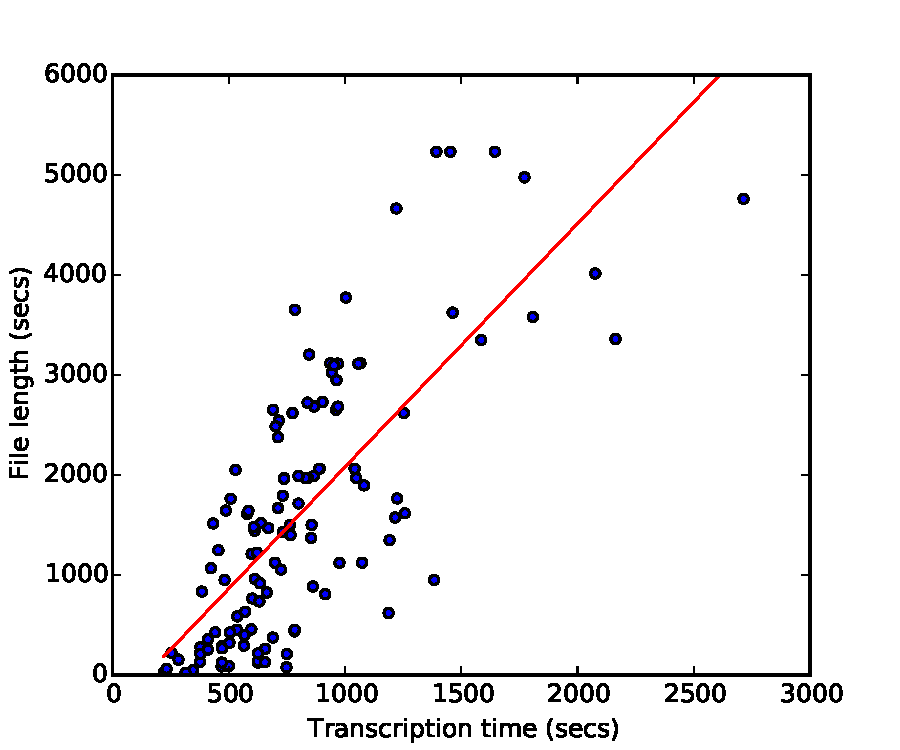
\includegraphics[width=\columnwidth]{figs/transcribetime.pdf}
  %\caption{Time taken to transcribe each recording with linear trend line}
  %\label{fig:transcribetime}
%\end{figure}

\subsection{System description}

This section gives a brief overview of Dialogger, including its functionality and operation.  A screenshot of the
interface and numbered list of the main features are shown in Figure~\ref{fig:interface}.  A live demo of the system is
also available\footnote{\url{https://speecheditor.virt.ch.bbc.co.uk/demo} (accessed 15.08.2016)}.

\begin{figure*}[ht]
\centering
  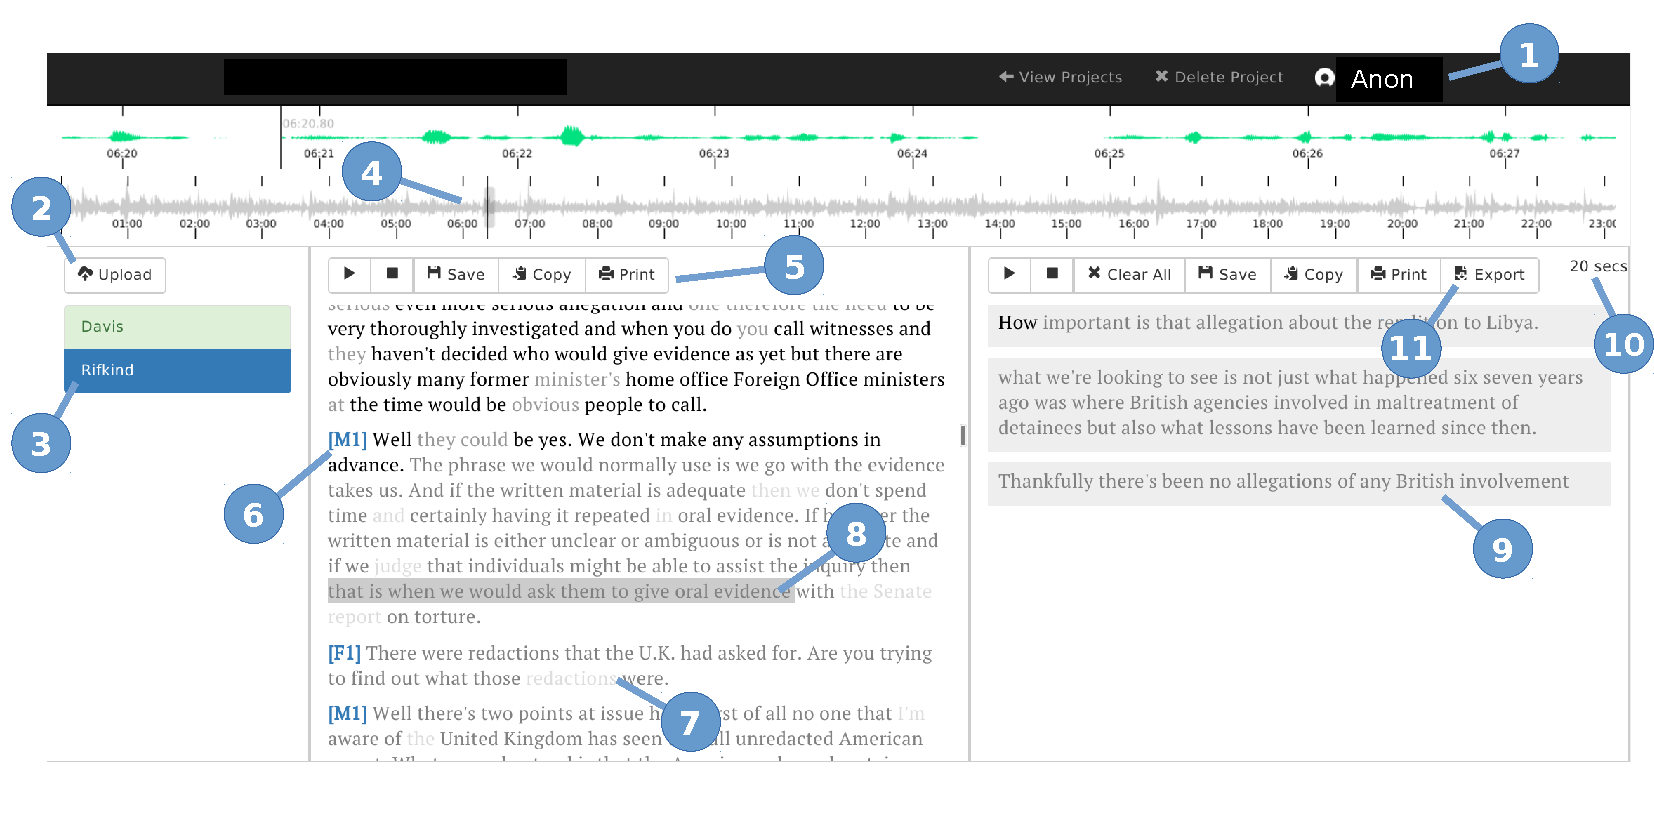
\includegraphics[width=\columnwidth]{figs/interface-labels.pdf}
  \caption{Screenshot of the user interface with highlighted features: (1)
    individual user accounts and projects, (2) upload of audio recordings, (3)
    list of uploaded recordings, (4) waveform display of currently selected
    recording, (5) toolbar with playback, save, copy and print functionality,
    (6) transcript of selected recording with speaker labelling and word
    editing, (7) confidence shading, (8) transcript selection with
    drag-and-drop editing, (9) listing and re-ordering of edits, (10) duration
    of edit, (11) export edit to audio file or digital audio workstation.}
  \label{fig:interface}
\end{figure*}

\subsubsection{Transcript}\label{sec:transcript}

The ASR system we chose was evaluated using a large multi-genre television dataset \citep{Bell2015}.  It had an overall
word error rate of 47\%, however for news content, which is clearly spoken by a native speaker, this dropped to 16\%.
As the speech on radio programmes is similar in nature to speech on television news, we found the error rate to be
comparable. However recordings with non-native speakers or significant background noise had a higher error rate.  For
comparison, the reported error rate of the system used by \citet{Whittaker2004} was 28\%, and for \citet{Sivaraman2016}
it was 10\%.

The time taken by the transcription service to process each uploaded recording was approximately half as long as the
length of the recording. The time depends primarily on the length of the recording but also on noise, accents and the
complexity of the speech.

%\subsubsection{Functionality}
%Dialogger is web-based speech editing tool that can be accessed from anywhere
%using a web browser.
%Users can upload their own speech recordings into a project in their individual user
%account. Each recording is automatically transcribed at around twice
%real-time speed, with a word error rate of approximately 16\%.

%The interface displays a list of the user's recordings on the left, the transcript of the selected recording in the
%middle, and a blank workspace on the
%right. The waveform of the selected recording is also shown at the top.
%Users can play a recording, and navigate it using either the transcript or the waveform.

%The transcript is divided into paragraphs at points where the speaker changes. Each paragraph is labelled with the
%speaker's assigned identity, including their gender (e.g. [M3]). Words that might not be correct are shaded grey, and
%incorrect words can be fixed by the user. Buttons at the top of the transcript
%allow the user to print the transcript, or copy it into a word processor.

%Recordings can be edited by highlighting and dragging words from the
%transcript to the workspace on the right, which creates a clip. Multiple clips
%can be created and re-ordered to produce an edited version. The edited version
%can be played to allows users to preview the result. The user can save their
%edit to revisit later.

%The interface displays the total duration of the edit. The edited version can
%be exported as either a .wav audio file, or as an edit decision list (EDL) for
%a digital audio workstation (DAW).

%TODO Add block diagram?
\subsubsection{Operation}

The functionality and operation of the system is described below as a typical user journey. Each feature is numbered
and shown in Figure~\ref{fig:interface}.

Users access Dialogger by navigating to a web page in their browser. They start by logging into the system using their
account (1) and create a project where they can upload their speech recordings (2) that appear in a list on the left
(3). Each recording is automatically transcribed. When it is opened, the waveform appears at the top and the transcript
appears in the middle section.  The recording can be played (5) and navigated by using the waveform (4) or by clicking
on a word in the transcript (6). The transcript shows where different people are speaking using paragraphs labelled
with the speaker's gender and an identification number (e.g. [F2]). Words which are likely to be incorrect are shaded
grey (7), known as `confidence shading'.  Incorrect words can be fixed by double-clicking them and typing the correct
word.  The transcript text can be copied or printed using buttons at the top. The audio can be edited by selecting a
range of words (8), then using drag-and-drop to place it in the area to the right which creates a clip (9).  Clips can
be re-ordered and deleted. The total duration of the edited clips is displayed (10). The edited audio can be played
through to preview the result, and the edit can be saved. Finally, the edited clips can be exported as a .wav audio
file or as an EDL (11) for further editing in a DAW.

%During this period there was no easy
%way to listen to the audio, so although they know \textit{what} was said, they
%don't know \textit{how} it was said.

%After editing using the transcript, the producer must go back to find and cut
%each piece of audio they wanted to use in the programme, known as a `rough edit'. Moving from audio to text and back
%again is costly, but is considered by the producers to be worthwhile. We believe that by linking audio and text
%representations together in a single editing system, it would be possible to
%work with either representation without incurring the cost of converting between the two.

%The pilot study also found that some of the functionality included in previous
%studies is already efficiently handled, or cannot yet be automated. For
%example, advanced music discovery platforms like Audio
%Network\footnote{\url{https://www.audionetwork.com/}} allow producers to
%quickly find music tracks of the right length, and removing `umm's or breaths
%from speech transparently is a skilled task that requires fine editing and
%human judgment.

 %It found that producers of speech radio prefer to work with
%text-based representations of audio rather than with the recordings directly.
%Their workflows are primarily paper-based which creates extra work when moving
%between paper and audio. Creating a link between the words on the paper and
%their location in the audio recordings could significantly improve the
%production workflow.

%The study also identified opportunities to apply semantic audio technology
%and interaction design to radio production tasks. Lots of time is spent
%cleaning up recordings by removing redundant speech, which could be fully or
%semi-automated. Segmenting speech content by speaker would make a positive
%impact on most speech-based tasks. Finally, drama productions could benefit
%from an easy way to compare multiple takes of the same scenes.

%\subsection{Design}
%We designed Dialoger to play to the strengths of transcript-based editing by
%focusing on the key features for logging and rough editing, and integrating
%well with the current production workflow. We excluded some features like
%removing `umm's or adding music, which are better handled by existing systems or techniques.  We also excluded
%detection and handling of repeated phrases, as this technique is only used in drama production.

%This section describes the design, features and implementation of the prototype.




%\subsubsection{Transcription} \subsubsection{Layout}
%The interface is laid out so that the workflow operates from left to right.
%Recordings are uploaded and listed on the left (2), the transcript of the
%currently selected recording is shown in the middle (6), and clips are created and exported on the right (9). The
%waveform of the currently selected recording is shown at the top on a dual time-line (4), where the bottom waveform
%shows the entire recording and the top is a magnified display of the current position.

%\subsubsection{Navigation} Users can navigate the selected recording by clicking on a word in the
%transcript, which seeks to that position and starts playback, or by clicking on
%the waveform to jump to a specific time. Playback can also be controlled using
%buttons in the toolbar above the transcript (5).

%The text before and after the current playback position is coloured black and
%dark grey, respectively, to indicate the current playback position in the
%transcript.  Words which the speech recognition system is not confident about
%are shaded in light grey (7), known as `confidence shading'.


%\subsubsection{Editing}
%An audio clip can be created from the transcript using drag-and-drop.  The user
%selects text from the transcript (8) then drags and drops the selection in the
%space to the right.  Each clip is contained in a shaded box (9) which can be
%re-ordered by dragging them up and down, or deleted by clicking an `X' in the
%top right of the box.

%The clips can be played using the playback buttons at the top, or by clicking
%on a word. The total length of the clips is displayed above the text (10).


%\subsection{Implementation}
%The system was implemented using web standards, which allowed a consistent
%experience on any recent web browser, and avoided the need to install any
%software locally. The front-end was written in Javascript using the Hyperaudio
%\citep{Hyperaudio} and peaks.js \citep{Peaks} libraries, and the back-end was
%built using Node.js and MongoDB running on a virtualised Ubuntu server.
%Communication between the two was done through a REST API.

\section{Evaluation methodology}\label{sec:methods}

We wanted to determine whether professional radio producers could successfully employ the features of Dialogger
as part of the production of a real radio programme. Specifically, we were interested in measuring
whether the system was faster than their existing technique, and if it continued to be used after the trial.  We also
wanted to investigate how the system was used and whether there were any features that could be added to improve the
functionality.

Additionally, we wanted to take this opportunity to continue our research on the existing radio production workflow to
learn more about the challenges producers face and the tools they use to produce their programmes. Our pilot study did
not explore requirements in-depth, and there is not much previous literature that analyses actual radio production
practice, so we wanted to be able to inform researchers and designers about real requirements and behaviour in this
field.

To achieve these goals, we conducted a qualitative contextual study of radio producers working under two conditions --
the existing editing workflow and the semantic editing workflow.

%\subsection{Research questions}
%The questions we aim to answer through this study are as follows:
%\begin{itemize}
  %\item What is the workflow used by radio producers to create a pre-produced radio programme?
  %\item What challenges do radio producers face in creating a pre-produced programme?
  %\item Which tools do radio producers currently use for editing audio, and how are they used?
  %\item Can a semantic editing system be used in the radio production workflow?
  %\item Do radio producers edit audio faster using a semantic editing system compared to their existing system?
  %\item When left with access to a semantic editing system, do radio producers continue to use it?
%\end{itemize}

\subsection{Approach}
Gaining access to radio producers can be difficult as there are not many of them and they are normally very busy. A
number of unrelated studies on television production systems have previously been conducted
\citep{Engstroem2010,Perry2009}, but we were unable to find any studies at all which used radio producers.
\citet{Kim2003} attempted to recruit radio producers but was unsuccessful because the producers were ``so highly
tasked''. However, in this case we were able to recruit professional radio producers from the BBC due to the access
available to us as an internal research department.

%To account for this, we designed our study to take place at their desk and to overlap as much as possible
%with the work they already need to do.
As we would not be able to recruit a large number of participants, we chose to take a qualitative approach to maximise
the depth of the information gathering. To take advantage of the available access to the work environment, we chose to
use contextual inquiry techniques to allow us to learn about the workflows, tools, and the social, technical and
physical environments. This took the form of an initial interview, followed by a period of observation, then a final
interview.

Radio producers find it difficult to step away from their day-to-day work for too long.  To account for this, each
system was used for the production of the programme that the participant was working on at the time, and the audio
content they needed to edit that day. Participants were interviewed and observed in their normal working environment.

\subsection{Design and procedure}
We designed a five-stage experimental procedure that followed a typical contextual inquiry format of
interview/observation/interview. In addition, we recorded some simple metrics such as task completion time and feature
usage.

\paragraph{Stage 1: Background interview}
    Participants were first given an overview of the project and the study, and asked to complete a consent form. This
    was immediately followed by a semi-structured interview to learn about the participant's background, their existing
    production workflow and the tools they used as part of that. The investigator asked participants to describe the
    radio production process in detail, and used follow-up questions to clarify their understanding. This information
    was recorded using written notes.

\paragraph{Stage 2: Dialogger training}
    A short training session on the Dialogger interface.  Each participant was trained on the interface's
    functionality using a pre-written `tool-tip tour', in which the participant was presented with a sequence of
    instructional pop-up dialog boxes overlaid on the interface.  This ensured consistency of training between
    participants. Each participant was then issued with a series of tasks that utilised all of the system
    functionality. The investigator observed this stage and wrote notes of any unexpected behaviour or stumbling
    blocks.

\paragraph{Stage 3: Task observation}
    Observing the participant as they produced a radio programme.  Each programme is composed of a number of interviews
    on a single topic, or set of topics.  We observed the participant while they logged and rough-edited two
    different interviews for the same programme. They did this by editing an interview under each condition -- one
    using their existing production workflow, and the other using Dialogger. The order of the conditions was
    counterbalanced.

    The investigator sat beside the participant during the task and wrote notes on the workflow, tools, generated
    metadata, usability issues, task completion time, and unexpected reactions or usage.
    The actions of the participant on Dialogger were logged electronically. After they completed the task, they were
    asked to rate each condition using the NASA Task Load Index metrics \citep{Hart1988}.

    %The tasks were performed as part of the production of a real radio programme,
    %and the observation was done in the participant's normal work environment.

\paragraph{Stage 4: Interview}
    A semi-structured interview about the participant's experience of each system and how they compared. The
    investigator questioned participants about the advantages and disadvantages of each workflow, then asked about any
    specific topics, issues or questions that cropped up during observation. The audio from this interview was recorded
    and transcribed to allow for further detailed analysis.
    %The questions asked were:

    %\begin{itemize}
        %\setlength\itemsep{0em}
      %\item Which aspects of the existing system did you / did you not find useful?
      %\item Which aspects of the prototype system did you / did you not find useful?
      %\item Overall, which system did you prefer and why?
      %%\item Did the prototype change the way you made the programme? If so, how?
    %\end{itemize}

\paragraph{Stage 5: Follow-up}
    Each participant was then given access to Dialogger for a further month, and was invited to continue to use it if
    they wished. Each week, they were asked via email whether they had been using the system, and if so, which features
    they valued most/least or were missing.  During this time, their usage of Dialogger was also logged electronically.

\subsection{Recruitment}

We invited professional radio producers with at least five years of experience to take part by sending an email to
departments in BBC Radio that create pre-produced factual programmes.  Drama programmes were excluded from the study as
their production workflow involves making multiple recordings of lines in a script and selecting the best ones
\citep{Baume2015}. This is a sufficiently different process to other programme genres that it warrants a different
interface.

Five participants (P1--P5) were recruited (4 male, 1 female) who each had between 6 and 20 years experience in working
as a radio producer. Although we had a small number of participants, the experience of the producers and the depth of
the study means that their feedback should carry significant weight. Five participants is also considered sufficient
for identifying most usability problems \citep{Nielsen1993}.

During the experiment, the participants worked on programmes of different
lengths from a range of genres:
P1 produced a single 27-min documentary, %plus 50-min for WS
P2 produced a 27-min documentary as part of a ten-part series,
P3 produced a single 45-min documentary,
P4 produced a 14-min archive programme
(based around material from the archive) as part of a ten-part series, and
P5 produced a single 27-min magazine show (covering multiple stories on a
single theme).

\subsection{Analysis}
The study produced a large amount of data, including observation notes, interviews and metrics. We used coding to
analyse the textual data and statistical analysis for the numeric data, as described below.

\subsubsection{Coding}
We manually transcribed the audio recorded from the interviews in Stage 4 to produce a verbatim transcript, and
collated them with notes made by the investigator from Stages 1, 2 and 3. To organise and process this textual
information, we employed the use of coding techniques.

We performed a two-stage coding process.  Firstly, we openly coded each part of the transcripts into a flat structure.
As there are not many previous studies on radio production, we decided to use open coding so that the categories would
emerge from the data we collected, rather than attempting to test an existing model.  We used the software package RQDA
\citep{RQDA} to execute this stage.

Once all of the text had been processed, we grouped the codes that had common themes. We used mind-mapping software to
help us re-arrange the codes into various hierarchical structures until a logical solution was found.  The coding
and grouping was performed by the investigator that collected the data.

\subsubsection{Metrics}
Although this was primarily a qualitative study, we chose to collect some basic metrics to measure task completion
time, cognitive load and usage after the trial.

We used task completion time from stage 3 as a metric for editing speed. As participants used different interviews of
varying lengths for each condition, we measured task completion time relative to the length of the audio
recording being edited. We used a paired \textit{t}-test to test for any significant difference between the existing
and semantic editing workflows.

To measure the cognitive load of each task, we used the raw TLX metrics gathered from the questionnaire in stage 3. We
used a paired \textit{t}-test on each of the six metrics to test them individually for any significant differences.

Finally, to measure the level of usage during the follow-up in stage 5, we collected the time spent using the
interface, the number of new uploads and the number of exported edits. As this data is only relevant to the semantic
editing workflow, the raw numbers will be reported.

\section{Results}

The coding process resulted in 40 codes, which were grouped into ten categories and four themes (see
Table~\ref{tab:codes}). The codes contain comments about both the existing and semantic editing workflows, however for
clarity we will present these results individually.

We start by going through the existing radio production workflow in detail, with an emphasis on the challenges that
were identified, and the tools that are used as part of the process. We then consider the semantic editing workflow and
expand on the four themes identified during coding. Finally, we look at the results of the metrics that we captured
during the observation and final follow-up stage.

\begin{table}[h]
\centering
{\small
\begin{tabular}{|p{0.18\linewidth}|p{0.2\linewidth}|p{0.5\linewidth}|}
\hline
\multirow{5}{*}{Comprehension}
 & Challenges & Complexity, quantity, environment, concentration, take taken \\ \cline{2-3}
 & Navigation & Speed, search, paragraphs, speaker segmentation, time since recording, cross-referencing \\ \cline{2-3} 
 & Accuracy & Correction, accents, good enough, confidence shading, use after editing \\ \hline 
\multirow{3}{*}{Organisation}
 & Mark-up & Bold, star rating, labelling, annotation, timestamps, word processing \\ \cline{2-3} 
 & Programme script & Structuring, collaborating with presenter \\ \hline 
\multirow{2}{*}{Editing}
 & Sound quality & Fast playback, anxiety of not listening \\ \cline{2-3}
 & Technique & Deleting, workflow, transcript not needed for short edits, similarity to TV \\ \hline
\multirow{3}{*}{Usability}
 & Portability & Laptop, paper \\ \cline{2-3} 
 & Drag'n'drop & Space on clipboard, scrolling \\ \cline{2-3} 
 & Misc & DAW integration, transcript turnaround time, simultaneous uploads, video support, waveform, avoidance of repetition \\ \hline
\end{tabular}
}
\caption{Topics, categories and codes (left to right), that emerged from analysis of the interviews in Stage 4 and the
observation notes from Stages 1, 2 and 3.}
\label{tab:codes}
\end{table}

\subsection{Existing workflow}\label{sec:resultsexisting}
%\subsubsection{Observation}
%During the first interview, participants worked with the investigator to
%identify a particular task in their workflow that would form the basis of the
%observation. In every case, logging and rough editing of an interview was
%selected, as this process takes a long time, is considered tedious and would
%benefit from automatic transcription.

%Due to the pressured and changing work environment, the observation had to fit
%around the editing requirements at the time of observation. This meant that P4
%and P5 did not do any logging during observation.

This section describes the existing radio production workflow. The process is documented as described by participants
in the interviews (Stages 1 and 4) and as witnessed by the investigator during the observation (Stage 3).  We start by
providing an overview of the workflow, then discuss the topics identified through coding.

\subsubsection{Overview}

This section describes the high-level production workflow for pre-produced content as described by the
participants. This is also represented by the numbered diagram in Figure~\ref{fig:workflow}, and the description below
uses numbers to make reference to each part of the diagram.

\begin{figure}[ht]
\centering
  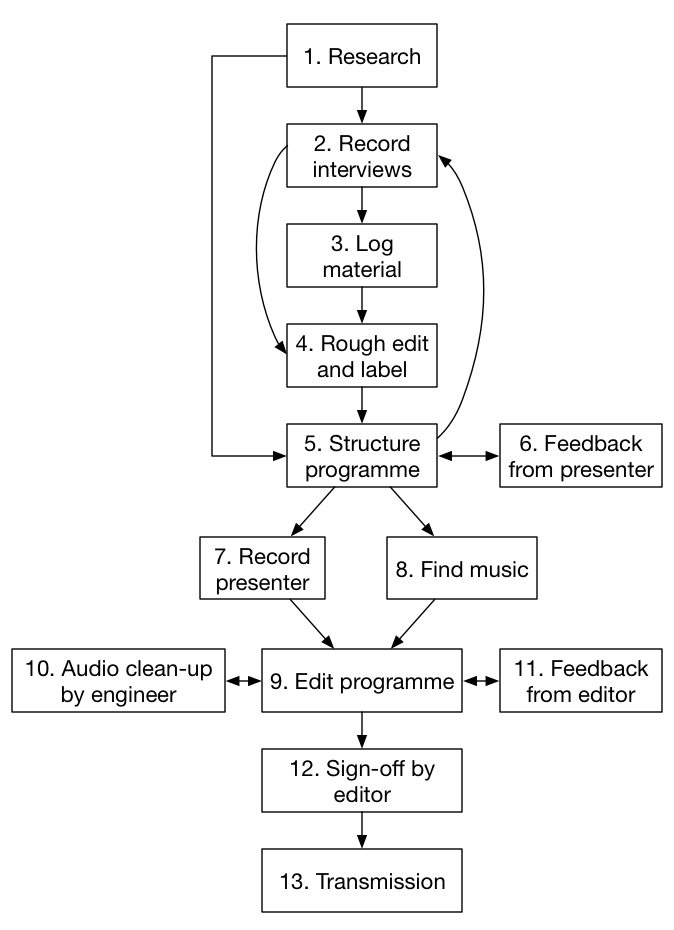
\includegraphics[width=.6\columnwidth]{figs/workflow.png}
  \caption{Radio production workflow as described by participants}
  \label{fig:workflow}
\end{figure}

When a programme is commissioned, the producer starts by researching the
subject (1) in detail to identify a compelling story and to find the best
contributors. This is done by reading, listening and watching existing material
on the subject, and finding and talking to relevant people. During this time
they also recruit a presenter for the programme.

After researching the topic, the producers then arrange interviews with
contributors and record them (2) with the presenter either in a studio, an external
venue or via a telecommunication link.

% Quote from P3
%Once you've got all the interviews recorded, before you start formally scripting and cutting the programme, you log
%them. You don't transcribe them precisely, but you do a rough transcription that is sufficient to copy those bits of
%text in to script, sufficient to find the bits of the audio you want to use and to make sense to the presenter.

Once material has been recorded, the next step is for the producer to select which parts of the audio they want to use
in the programme.  This selection process is often aided by creating `logs' of the interviews.  Logging (3) helps the
producer by allowing them to see, on screen or on paper, what was said in each interview, when and by whom, without
having to listen to it.  This allows them to quickly find and share the pieces that they want to use in the final
programme.  It also helps them structure their thoughts, identify themes running through discussions, and make links
between different interviews.

\begin{figure}[ht]
\centering
  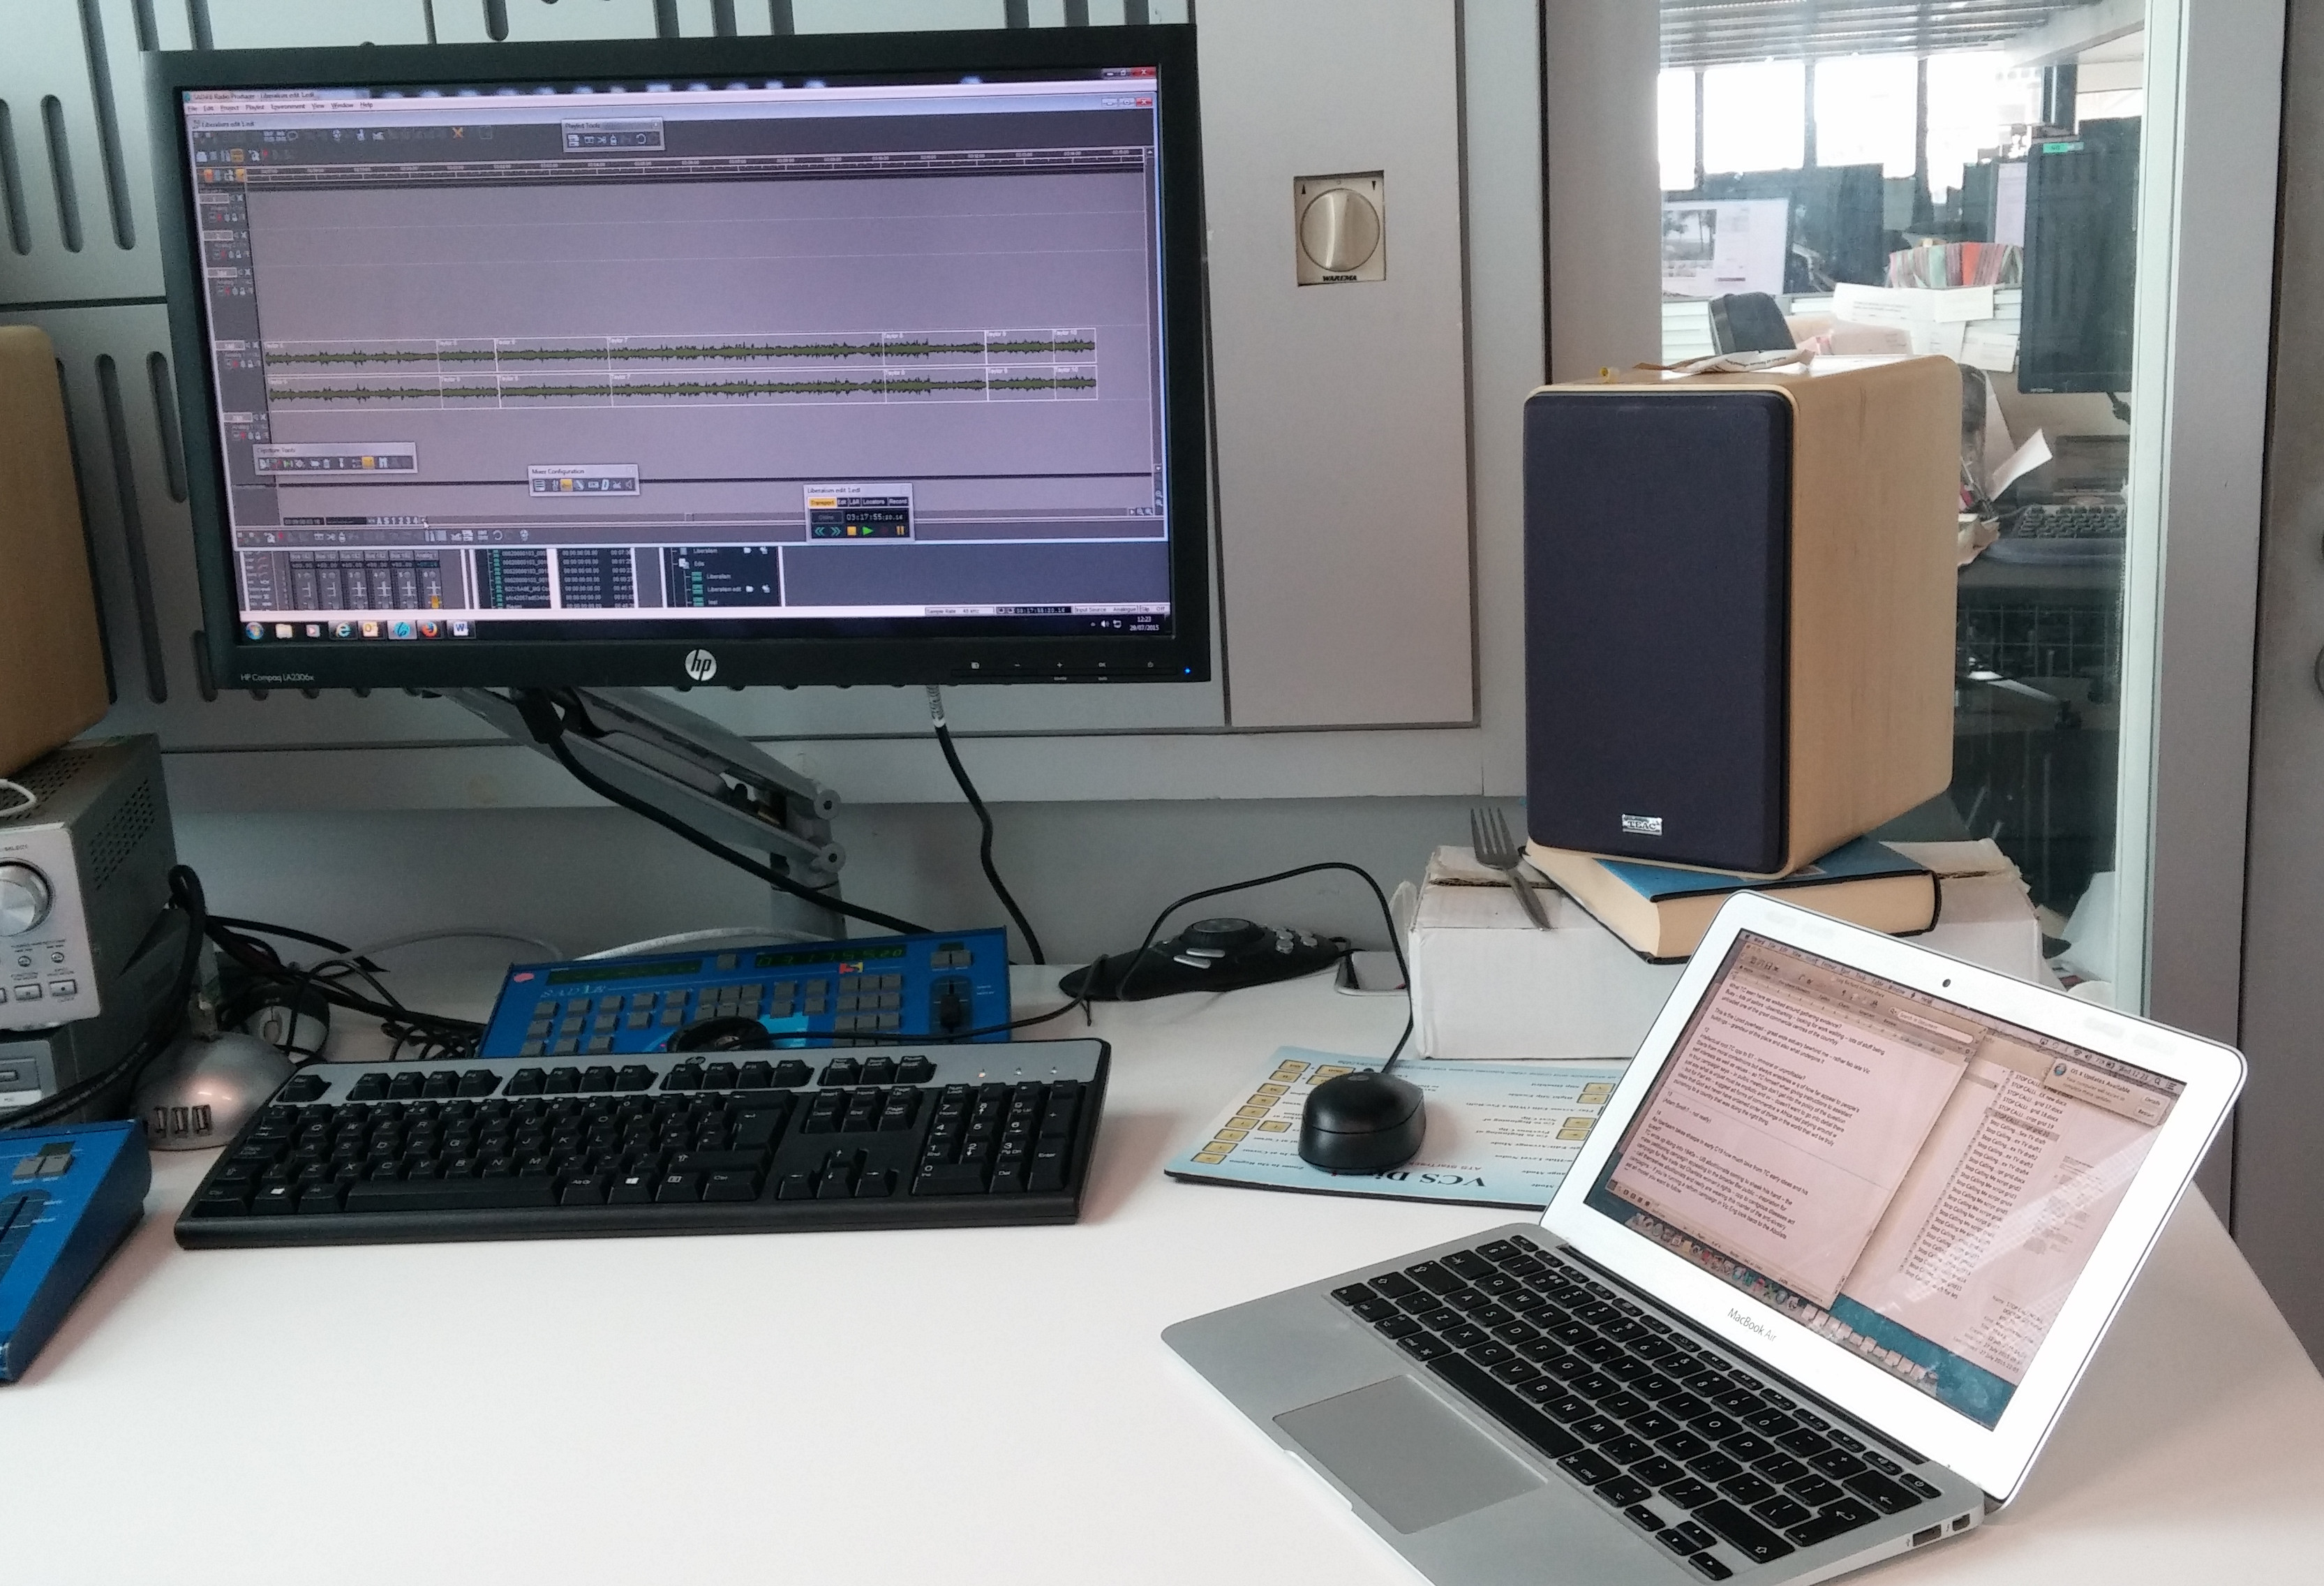
\includegraphics[width=\columnwidth]{figs/phil-desk.jpg}
  \caption{P3 logging interviews with a digital audio workstation on the desktop
    PC and word processor on the laptop}
  \label{fig:desk}
\end{figure}

Logs are usually written by the producer themselves. As they have done the research and are normally present at the
recordings, they can use their memory to navigate the material and use their experience to quickly determine which
parts are relevant. Some programmes that are under particular time pressure will use a third-party to create a verbatim
transcript of a few interviews \citep{Baume2015}, but most do not because it is too expensive.

In the observation, P1 and P3 wrote their logs in Microsoft Word whilst using a digital audio workstation (DAW) to play
the recording (see Figure~\ref{fig:desk}). P5 reported that they usually followed a similar process, but did not do any
logging during observation.

The exact format of the logs varied between individuals, but they usually contained a rough transcript of the interview
with occasional timestamps and notes. They reported that this helped them to find important bits in the recording later
on. Each producer has their own syntax, but there are commonalities.

Timestamps were written on the logs, approximately \textit{``every 30 to 120 seconds''} (P1) with minutes and seconds
in parenthesis: \texttt{(4'20)}, for example.  This allows the producer to navigate to a particular piece of audio much
faster than they would otherwise by narrowing down their search range.

The next stage is to rough edit (4) each recording, which involves segmenting the audio into chunks, removing the
chunks they don't intend on using, and to label and arrange the remaining chunks.  The editing reduces the amount of
material they need to work with, and the labels make it easier to identify which parts are which.  If a recording is
short (around 15 mins or less), then this process is usually done without logging the content first.

This process of recording, logging and rough-editing is repeated until the producer has enough material for their
programme. Throughout this process, a script is used to organise and structure (5) the content of the programme.  The
script usually takes the form of a Microsoft Word document, but can also be written on paper. Some producers only write
a rough outline, whilst others will copy in full transcriptions of the content they are using.  Some producers have an
idea of what the programme will look like before they make any recordings, so will create the script first. Others will
be guided by the content of the interviews, so will wait until they have some recordings before creating a script.

\textit{``As I'm organising a programme, booking interviews, talking to contributors, and planning interviews, I'm all
the time assembling a scratch structure that will eventually be the script.''} (P3) % It's not set in stone unless it
has to be

The script is also used to collaborate with and get feedback (6) from the presenter.  Using a written document rather
than audio files makes it easier to quickly review the content of the programme, make notes and suggestions, and to do
this over large geographic distances. The presenter uses the document to write and insert `links', which are the
narrative elements spoken by the presenter to link the interview clips into a story. They also insert comments and
notes for the producer. Once the script is nearing its final stages, the presenter records (7) their links and sends
them to the producer.

If the programme is part of a series, it will often have theme music. Any other music is chosen (8) by the producer,
often using production music services such as Audio Network\footnote{\url{http://audionetwork.com} (accessed 28/4/17)},
or the BBC's Desktop Jukebox.

Once the interview, links and music are ready, the producer will assemble these into an edit (9) that matches the
script, using the DAW. This edit will be about twice as long as the final programme, sometimes significantly longer
(e.g. P5 reported that they once created 22-hour-long rough edit for a 37-min programme). The producer then continues
to edit the audio, primarily to `get it down to time', but also to give it a final polish by cleaning up the audio.
Cleaning involves finely adjusting sound levels to be consistent, removing ``umm''s and breaths, and adding non-speech
sounds to create a rich auditory scene.  Producers who are skilled at using a DAW will usually clean up the audio
themselves, but others will bring in a sound engineer (known in the BBC as a `studio manager'), to help with this (10).

Before a programme is broadcast, it must be signed-off by the department head, known as the `editor'. Most producers
will get feedback from the editor (11) before this, so that they have time to make any requested changes. Often this
happens a day or two before transmission. Some participants reported that they sit in the room with the editor while
the current version is played, while others sent an audio file to the editor to listen by themselves. In both cases,
the editor gives oral feedback and suggests changes.  Once the editing is complete, a final version is rendered to an
audio file and added to the playout system for the editor to sign-off (12).

% Quote from P3
%So once you've got that done, you then start using your structure to assemble sound, assemble scripts, write links to
%go with those bits of transcript in the structure as it becomes a script. 

% Quote from P3
%The way I do it is that I have a piece of paper with the names of the sections, the rough amount of time I'm budgeting
%for each one and once I've done an assemblage of the amount of time I've got of each one I can see I've got 37 mins for
%part one where actually I need 4 mins and that motivates you to crunch it down. You just keep going round and round and
%round that until you get something that's coherent, clear and to time.

%\paragraph{(7) Record presenter} The next stage is to add narrative elements, known as `links' to join the clips
%together into a storyline. The producers reported that they work with their presenter to write the links together,
%using the programme script to collaborate. The presenter records the links in a studio and the producer then assembles
%them into the edit.

\subsubsection{Comprehension: Challenges}

The skill of the producer is to \textit{``separate the wheat from the chaff''} (P1, P3, P4 -- all verbatim) and to find
the clips which will make an interesting programme.

\textit{``That's the basis of my job - to find great stuff and put it together.
  It's not difficult putting it together, it's finding the great stuff and finding connections between it. Getting rid
  of the non-great stuff is
  challenging and time-consuming, and it requires mental processing.''} (P1)

However, the sheer quantity of recordings means this process adds significant overhead.

\textit{``you've got an average of 45 mins per interview and in a series of
  three programmes you've got seven per programme, that's a lot of work''} (P3)

Interviews recorded for speech radio often cover complex topics in fine
detail. Keeping track of all the points raised and forming a compelling
narrative from them is a challenge.

\textit{``All the interviews overlap with each other terribly, and have got
  similar themes.''} (P4)

Writing the logs takes a lot of concentration as the producer must listen to
what is being said, work out how it ties in with other contributions and the
story, and make swift judgements on whether it should be used.

\textit{``one of the slightly exhausting things about doing it is the level of
  concentration you have to maintain to make good decisions, remember where
  everything is, what you've got, is kind of strained rather by having to just
  do schleppy tasks like moving the sound and logging interviews''} (P3)

P1 and P5 reported that they find the office environment distracting, so often work at home or outside the office.

\textit{``I typically do this at home because I find it a much less distracting
  environment. It does require quite intensive concentration so you don't miss
  something.''} (P1)

%Quote from P5
%Where I find it useful is when I'm away from the office and away from the machine, and that sort of thinking time
\textit{``In the office there's so much pressure and you're always doing stuff.''} (P5)

Although P4 did not do any logging during observation, they explained that for longer recordings, they
would normally write logs by hand in a notebook whilst listening on a
portable music player somewhere away from the desk, such as in a caf\'e.

The high level of concentration required, combined with the repetition of 
typing and listening to the interview again means that producers need to take
regular breaks.

\textit{``it's boring and it's not very easy to be efficient at it [...] when
  I'm normally doing it I'm checking my emails, making a cup of tea.''} (P3)
\subsubsection{Organisation: Programme script}
The producers organised the programme by writing a `script'. This is primarily used to help them structure their
thoughts, but also to help communicate with the presenter over email.

%The scripts contain varying amounts
%of detail, depending on the subject and the individual producer. Some will
%eventually include a full transcription of the programme, whilst others will
%remain as a bullet-point outline.  The scripts are written using Word, with P2
%also using `MindManager' mind mapping software.
%The script can be created at any point during production, but is often started
%during the research stage.
In the study, P1, P2 and P5 started their scripts during the research stage by writing an ordered list of bullet points
of topics to cover and a list of draft questions to ask contributors.  P3 and P4 waited until after they had done some
interviews to start the script, as they wanted to structure the programme around the discussions that they recorded.

P3 and P5 updated the script after every edit to ensure they were always in sync. This added significant overhead but
gave them a visual structure to follow when making the final changes.
Having an accurate script also makes it easier to re-use the programme afterwards, when creating another version of a
different length, or for pulling out clips for the website.

%\textit{``What was really good was being able to take the final script that I had typed up as I was editing and tie it
  %to the finished programme in the system.
\textit{``[The script] is going to be invaluable when it comes to re-cutting this.''} (P5)

\subsubsection{Organisation: Mark-up}

P1, P3 and P5 would make comments for themselves in the log to help them when
editing. For example, ``\textit{[good to here, dull after]}'' or
``\textit{[trails off 9'30]}''. P1 also used a star rating system to rate the
quality of each point, for example ``\textit{[**** should use this stuff, but
  dramatically cut down]}''.

\textit{``What I sometimes do when I edit are star good bits, and I think
  that's quite a common trait.''} (P3)

Bold highlighting was also used by P1 and P3 to mark bits of the transcript
which are important and worth keeping.

\textit{``what I did was just put in bold the paragraphs I thought were worth
  [keeping]''} (P1)

P2 used a different approach to logging their material. Instead of logging the material by writing a transcript, they
played the recording in a DAW and used a keyboard shortcut to create timed markers at any points of interest. By seeing
where the markers clustered, they identified where to make clips, then gave each of the clips labels. This approach
allowed them to focus more on the audio, but didn't allow them to make any detailed notes.

\subsubsection{Editing: Sound quality}\label{sec:existing-quality}

Radio is an audio-only medium, so the quality of the content is highly dependent on the quality of the sound.  The
criteria producers use for deciding whether a piece of audio is good enough to use in their programme is not just about
what was said, but how it was said and how well it was said.

\textit{``How people say things is very important.''} (P5)

On the one hand, producers need to listen out for any poor quality sound that might negatively affect the programme,
such as people mumbling, stumbling, coughing, or any excessive background noise. 

\textit{``I've done paper edits before where I've gone back to that bit of audio and they didn't quite finish the
  sentence or they muttered it. You just couldn't use it at that point.''} (P3)

However, the producers were are also listening out for anything that worked particularly well, such as a moment of
comedy or passion, or a sound that perfectly captures the right feeling. Identifying these using the text of a
transcript is very difficult or impossible. 

Every participant that performed logging played the audio faster than real time at least once. This allowed them to
efficiently listen out for anything they might want to use while reviewing parts of the interview that may not be of
interest (e.g. off-topic or `off-mic' discussions).  P2 also used faster playback to prevent themselves from
over-thinking their edit decisions and picking out too much material.

\textit{``The ability to listen at faster than real-time [...] gives me the opportunity to come to a swifter decision.''}
(P2)

%\textit{``There's quite a lot of judgement I've got to make just on what the listening quality is.''} (P2)

\subsubsection{Editing: Technique}

If the recording was short and had been recorded recently, as was the case for P4 and P5, it can be edited
without first creating a log.

\textit{``If it's a quick ten minutes with three questions, you don't need to bother''} (P3, also P4 and P5)

In this situation, we observed that the producers listened through the recording using a
DAW and pressed a keyboard shortcut to split the recording, usually at the beginning/end of questions/answers. They
then went back to remove unwanted segments and add labels to the remaining ones.

In the cases where the recording was logged (P1, P2, P3), the producers used the log to decide which parts to select or
remove. They used the timestamps written in the log to narrow down their search area for each clip they extracted.
However, even with a reduced search area, the producers found it time-consuming to find the exact start and end point
of each clip using the DAW interface.

In the study, three of the participants (P3, P4 and P5) used SADiE as their DAW, which is provided to the producers by
the BBC. However, the other two participants chose to use other software packages that aren't formally supported. P1
used Adobe Audition because they were familiar with the interface and it was installed on their laptop, unlike SADiE
which was only available to them on a desktop computer.

P2 comes from a television production background and used Apple's Final Cut Pro, which is primarily a video editor but
also includes audio editing functionality.  P2 used Final Cut Pro because they were familiar with the interface and had
it on their laptop. In addition, they enjoyed being able to import audio directly from video content without having to
use another program to extract the audio first, and being able to use the video `titles' feature to make written notes
that can later be viewed in time with the audio.

\subsection{Semantic editing workflow}\label{sec:resultsnew}
This section discusses the results and themes that emerged from the evaluation of the semantic editing interface.
Participants were first introduced to Dialogger through a training stage (Stage 2). All of the
participants completed the training without any major issues. However, this stage highlighted a requirement for
keyboard shortcuts which was not previously identified.  P2 and P3 kept trying to use the space bar to start and pause
audio playback. This is a common shortcut in most DAWs which these participants naturally reached for. Reports on
previous semantic editing systems have not mentioned keyboard shortcuts, however they could be used to assist the
editing process.

In the rest of this section, we will discuss each of the themes that came out of the coding (see Table~\ref{tab:codes}).

%To evaluate the semantic editing interface, participants were observed while
%they used the system to log and rough edit recordings for a programme.
%Although it was designed as an all-in-one solution for putting together a rough
%edit for a programme, participants used the interface in different ways to
%integrate with their existing workflow.

%P3, P4 and P5 used the interface much as designed by using the transcript
%window to read and identify suitable clips, then dragging them across to the
%edit window and exporting the audio.


%P1 completed the test quickly and without issue,
%expressing that it was easy and intuitive. The other four participants
%successfully completed the test, but identified a number of minor usability
%problems regarding keyboard shortcuts.

%Two of the five participants (P2 and P3) kept pressing the space bar to start and pause audio playback. This may be
%habitual, as it is a universal keyboard shortcut in all DAWs. However, this feature was not considered when designing
%Dialogger.  Additionally, P2 tried to use word processing shortcuts in the
%interface, such as Ctrl+C and Ctrl+V to copy/paste and backspace to delete.

%P1, P2 and P4 reached for Ctrl+F to search for a word they were looking for. Although this feature wasn't explicitly
%implemented or mentioned in the training, the functionality was included in the browser. The participants remarked
%that it was a powerful tool for navigating the recording.

%In conclusion, we found that keyboard shortcuts are more important than we had
%considered when designing Dialogger.

%The interface was designed to allow users to copy the text of the entire
%transcript by pressing a `copy' button. Four of the five participants
%intuitively selected the text before pressing the copy button.  P2 expressed a
%preference to use Ctrl+C and Ctrl+V shortcuts to copy and paste text, rather
%than a drag-and-drop gesture.  Additionally, P2 said they wanted to be able to
%remove selected text by pressing backspace, or to export only selected text.
%Future versions should
%consider allowing users to apply actions only to selected text.

%Three of the five participants (P2, P3 and P5) couldn't remember the action to
%correct a word (double-click). Two of them (P2 and P3) right-clicked the text
%and looked for an option in the context menu.

%P2 confused about double waveform

%\section{New workflow}
%Following the usability study, participants were observed using the prototype
%interface to complete a common production task and interviewed about it
%afterwards. This section documents the findings.

\subsubsection{Comprehension: Navigation}

Participants reported that having the transcript available in the semantic
editing interface allowed them to read and search the recordings much faster
than they normally would with a waveform, which is in line with previous findings from
\citet{Whittaker2004} and \citet{Yoon2014}.

\textit{``with having a transcript you're able to immediately scan through it
  10/15 times faster. Maybe that's an exaggeration but it feels ten times
  faster''} (P1)

The transcripts also allowed the participants to quickly cross reference what
was said in various interviews without having to listen through multiple times.

\textit{``where I'm picking shorter clips, making a point and moving on or I'm
  developing an argument between different people and cutting between them, it
  feels a lot more easy to construct that `on paper' than what I'm currently
  doing''} (P2)

%\textit{``If it's a shorter thing I'll bang it straight into SADiE and start
  %editing down to find the wheat from the chaff''} (P4)

Being able to click on a word to navigate to that point in the audio also
enabled the participants to use visual search to quickly find and listen to
bits they were looking for.

\textit{``you can do that with your eyes even quicker - zone straight in on the bits and that click to go  `that bit',
  `that sentence there', `that word there' ''} (P4)

Participants reported that editing with a transcript was primarily useful when working at the sentence level. When the
granularity of editing involves removing individual words, ``umm''s or breaths, they said that the DAW software is much
better suited to these tasks. This supports our design decision to integrate with DAWs.

\textit{``the real editing work actually happens after this has passed its main
  point of usefulness''} (P3)

%\textit{``I was using some interviews, some contributors recorded on one
  %ocassion, but across several programmes, several episodes in a series, or for
  %several different stories.''} (P4)

%\subsection{Navigation speed}

%\textit{``it took me 15 mins to read 35 mins and not just read, but read and mark
  %up''} (P2)

%\subsection{Time since interview}

%\textit{``you're kind of doing a paper edit on the basis of having recently
  %heard the audio''} (P3)

%\textit{``a lot of that guesswork was coming from the memory of being there at the recording... realising which bits
%were the questions from the presenter and which bits were answers.''} (P2)

%\textit{``I know I've got a doc coming up in six months time, so I'll ask them
  %some questions for that. Now then in six months time I can't remember what
  %the answer was''} (P4)

%The primary benefit of reading over listening is that you can quickly scan ahead and jump around with your eyes,
%whereas listening can only be done at a fixed pace. 

\subsubsection{Comprehension: Accuracy}
When using the semantic editing interface, editing decisions are based on an
automated transcript which is only partially accurate. Previous research has shown that for editing
voicemail recordings \citep{Whittaker2004}, discussions \citep{Sivaraman2016} and spoken comments \citep{Yoon2014},
automated transcripts were considered sufficiently accurate. However, the ASR transcript accuracy required for
navigation and editing in radio production is currently unknown.

The participants in our study suggested that the transcripts were, generally speaking, sufficiently accurate for their
purposes.

\textit{``It's clearly not 100\% in word recognition but I'm feeling it's
  certainly good enough for my rough cut purposes at this point''} (P2)

If the recording being edited was made recently, the producer can use their
memory of what was said to make sense of the inaccuracies in the
transcript.

\textit{``Both these interviews [being edited] are relatively recent so I have
  it reasonably in my mind what they've been saying. I was able to read roughly
  what there was - `okay that's that question', `I know what was in that
  question' ''} (P1)

In the existing radio production process, transcripts are used to aid the producer and presenter, but are
  not shared outside of the production team. In our study, the producers we observed only used the transcript
  to navigate and edit the audio. However, P3 and P4 noted that they were interested in correcting the transcript later
  so it could be shared or published.

\textit{``I'm probably posting transcripts for the whole interview. So I do
  need to go through and correct''} (P4)

Being able to provide corrected transcripts has the potential to make an impact beyond improving the
  editing workflow. For example, transcripts of the finished programme could make the audio content searchable and
  re-usable for print media.

%Clearly, the more accurate the words in the transcript are, the less work has
%to be done to correct it.

%\textit{``The closer it can be to the point where you don't have to clean it up
  %the better obviously, and that's quite significant honestly, that's my only
  %qualm''} (P3)

%Sometimes a word is commonly mistranslated throughout the transcript, so
%providing an easy way to fix that would be a useful addition.

%\textit{``Something that would be even better is Ctrl+H  replace function''} (P3)


%\section{Speaker diarization} One disadvantage of working with transcripts is that you can't hear which person is
%speaking when.

%\textit{``if you can't see who's speaking - that's a disadvantage''} (P3)

%Speaker diarization technology \citep{AngueraMiro2012} can be used to try and
%identify where different people are talking. The prototype included a
%rudimentary system that attempted to distinguish speakers and guess their
%gender, however it tended to significantly overestimate the number of speakers
%which caused some difficulty. 

%\textit{``It was distracting if anything, partly because I was trying to guess
  %who was which at certain points''} (P2)

%However, in many situations the participant could tell who was who from what
%they were saying.

%\textit{``It's reasonably clear to me who's asking the questions, but actually
  %[speaker diarization] is helpful''} (P1)

%During the study it was discovered that many producers record in stereo and use
%the waveform to see where people are speaking.

%\textit{``I always pan the presenter on one side and the contributor on the
  %other so I can see where the questions are''} (P5)

%This workaround could be exploited to improve the performance of a more
%advanced speaker diarization system.

\subsubsection{Organisation: Mark-up}
%Before creating any clips, P1 immediately copied the transcript text into Word
%in order to allow them to make annotations.

%The WAVs were then imported into the DAW
%by dragging and dropping them from the file system.

%In the observation stage, it was identified that annotation is an important
%part of the production process that was missing from the prototype.

During the study, P1 and P3 copied the transcript text from the interface into Microsoft Word. They
reported that they did this because there was no annotation functionality
available within Dialogger.

They inserted paragraph breaks, added notes after paragraphs, and
highlighted desired parts of the transcript in bold. Once the transcript was
annotated in Microsoft Word, they went back to Dialogger, found the parts of the
transcript they wanted by scrolling though the text, then dragged and
exported each clip individually as a .wav file.

\textit{``it would be better to take raw lumps of transcripts and plonking them
  in Word because Word has higher functionality than this''} (P3)

Producers are very familiar with the Microsoft Word interface so a later version of our
system could seek to provide a similar interface. This would allow producers to make annotations in the same way they
do already.

\textit{``With text editing, the reflexes are very much Microsoft Word''} (P4)

The most basic feature that could be added is highlighting, which is often used to note parts of interest

\textit{``If you just put a little star or underline or something simple to
  mark things, that would be a big gain for a small change''} (P3)

%\textit{``sufficient to find the bits of the audio you want to use and to make
  %sense to the presenter.''} (P3)

%\subsection{Star rating}

%\textit{`` I just gave myself a detailed breakdown of what was said in the
  %interview with timecodes at questions or major new points and a slightly
  %arbitrary scoring system to say 'that's really good stuff and must get in'.
  %''} (P1)

\begin{figure}[t]
\centering
  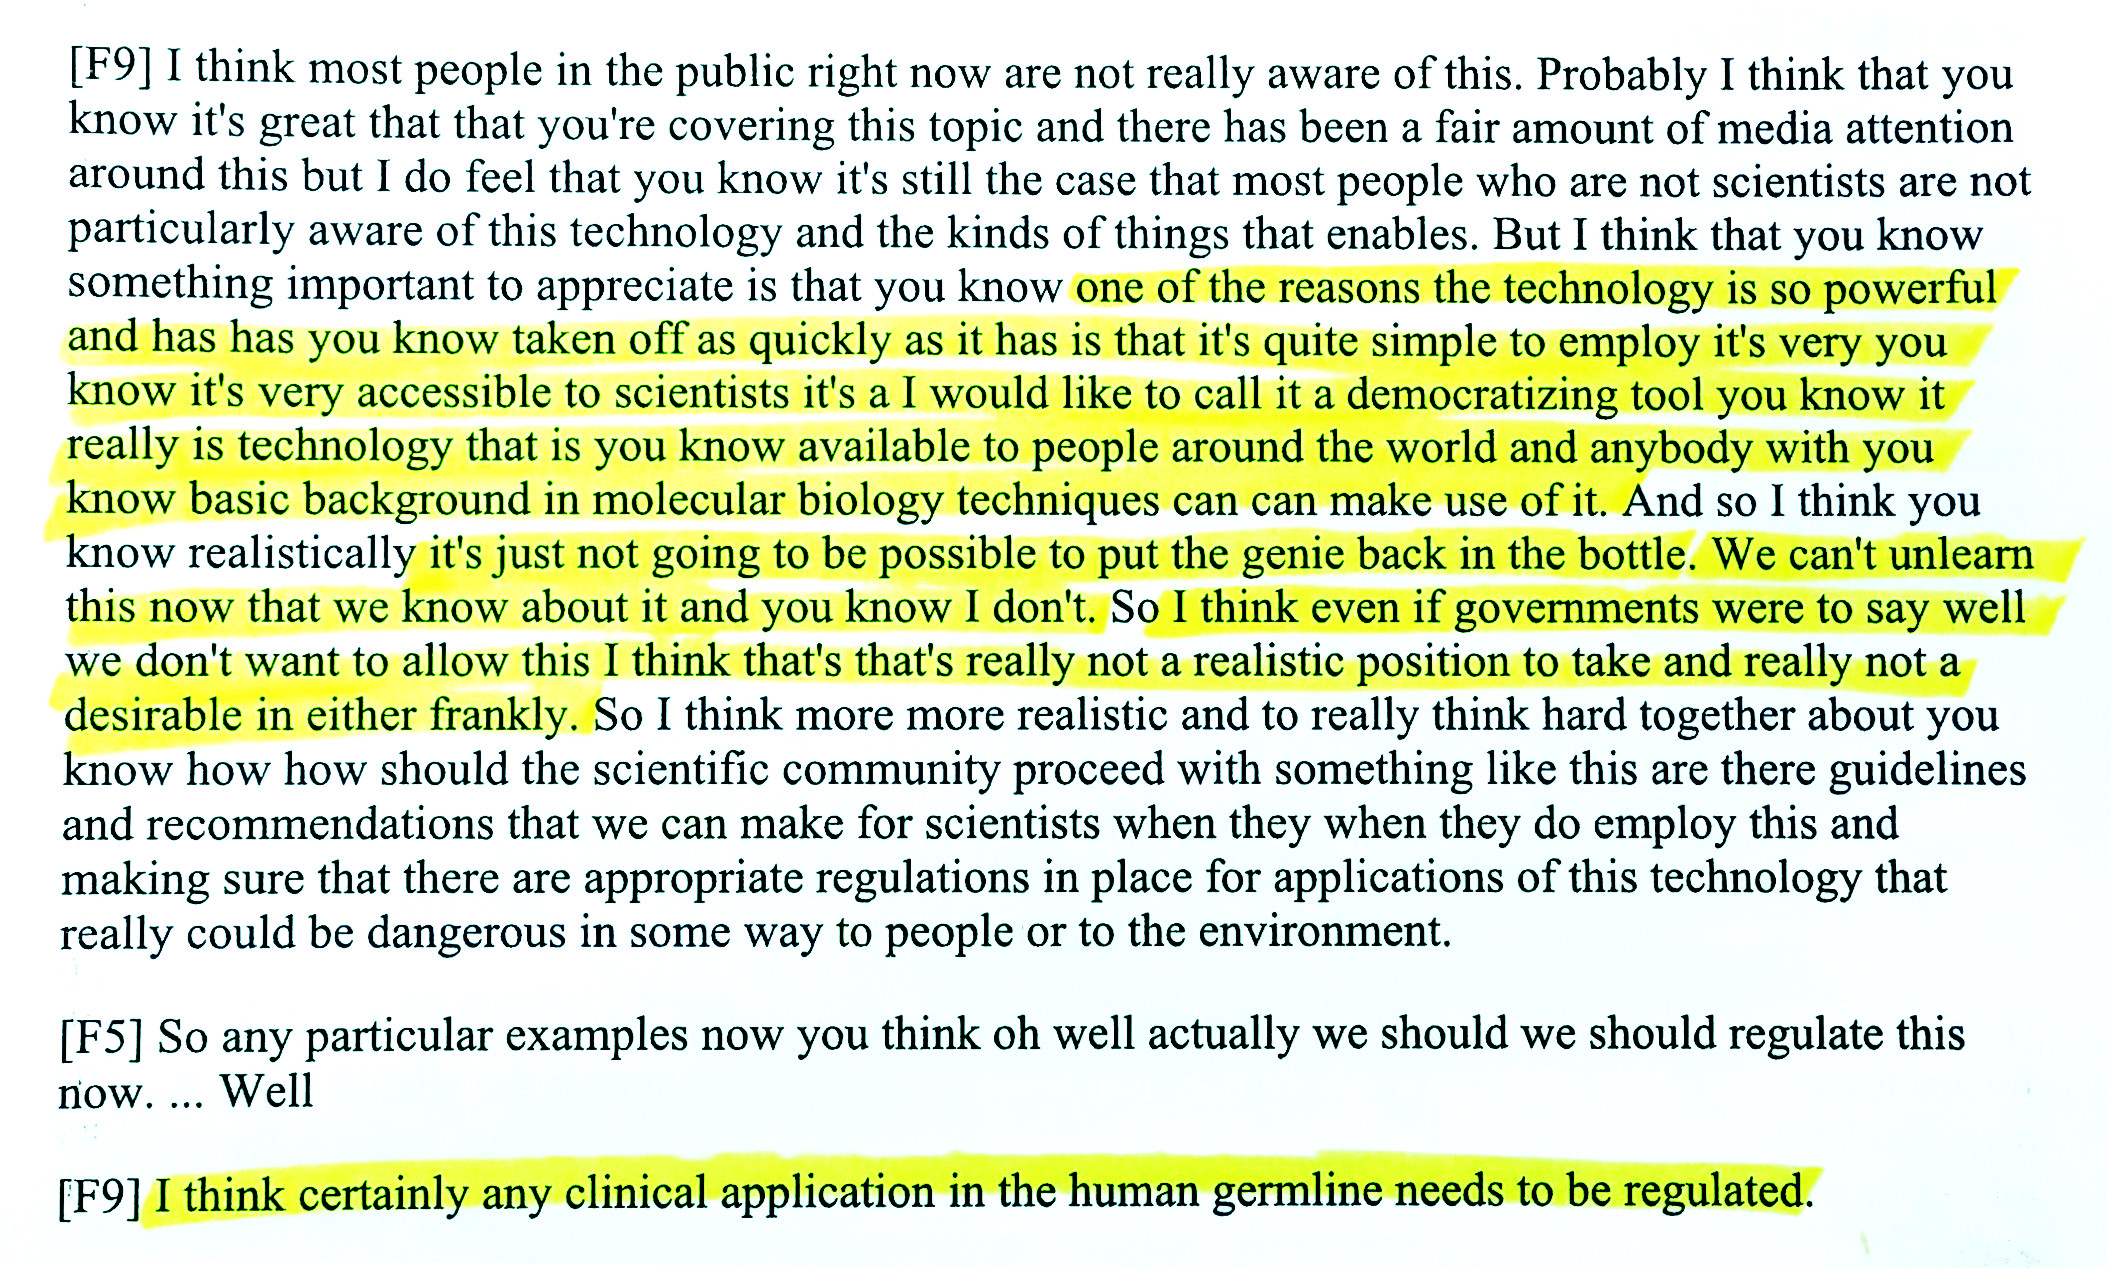
\includegraphics[width=\columnwidth]{figs/highlighting-cropped.jpg}
  \caption{P2 using a highlighter pen with a printout}
  \label{fig:highlight}
\end{figure}

\subsubsection{Usability: Portability}

P5 reported that working on paper allowed them to be productive outside of
the office, such as during their commute.

\textit{``What would be really useful would be to [...] take it away (say when
  I'm on the train going home) and I would paper edit the bits that I need''}
(P5)

Additionally, working on paper allows them to work anywhere as it does not
require electricity.

\textit{``It's highly portable. It doesn't require any power.''} (P2)

In the observed task, after uploading their recording, P2 immediately printed
the transcript and read through it on paper so that they could work away from
the screen.

\textit{``I'm reading a lot of material for a sustained period so I'd prefer to do it on page than on screen. Just
  easier on my eyes.''} (P2)

% Quote from P5
%you want to get away from the screen at some point

P2 then used a highlighter pen to select the desired parts of the recordings (see Figure~\ref{fig:highlight}).  After
highlighting all the pieces they wanted,
they then used the Ctrl+F text search to find the highlighted words in Dialogger.

\textit{``it allowed me to get to clips very quickly from a reference point on a printed transcript''} (P2)

However P2 noted that having timestamps on the printout may be a faster
way of achieving the same thing.
Once they had found and clipped all of the highlighted parts in Dialogger, they exported the clips into SADiE.

P4 explained that for an upcoming programme, they were
planning to print out transcripts from Dialogger to help
them collaborate with their presenter.

\textit{``we're just going to go through it with a pencil and paper, with a
  printout, and highlight the bits we want and cross out the bits we don't.''}
(P4)

\subsubsection{Editing: Sound quality}
Part of the appeal of having a transcript is that it frees the user from listening to the audio in real-time. It also
allows users to work on paper, away from any electronic devices. However, disconnecting the audio from the text
fundamentally changes the production process.

\textit{``Radio is made with your ears. You'll never get away from that fact that you need to listen''} (P4, also P2,
P3, P5)

There was also concern that parts which sounded great but didn't come across as well in the transcript may have been
overlooked.

\textit{``I was anxious it might not have sounded as good as it read, or that I might be missing bits that sounded
  great ''} (P2)

As discussed in Section~\ref{sec:existing-quality}, the participants existing workflow includes playing the audio
faster than real time, but that feature was not included in Dialogger.  Several of the participants noted that they
would like to have this feature added.

\textit{``it's a little bit annoying that there's no facility for that.''} (P2)

Although faster than real time playback normally reduces intelligibility, this may be less of a problem if the
transcript was available.

\textit{``you do still need to listen through, even though you've got the text.  Therefore, it would be optimised if we
  could listen through quickly''} (P4)

As listening is an important part of the production process, semantic audio interfaces would benefit from providing
easy access to the underlying audio to allow multi-modal interaction. Once the link between the audio and the text is
broken, re-linking the two together can be costly.

%\textit{``It's not very good at spotting breaths. You're always going to need [a DAW] for the fine edit.''} (P4)

%\textit{``Actually listening through to what sounds best, what is better audio, more entertaining inflexion of speech
  %rather than what is the content of those words. Those sorts of things you obviously can't tell from the written
  %page''} (P4)

\subsubsection{Usability: Drag-and-drop}

In Dialogger, we used a drag-and-drop technique for users to create clips from various interviews and
re-order them in a clipboard area. All of the participants were able to use this successfully, however we quickly
encountered issues when dealing with longer clips.

\textit{``I found the interface quite clunky for pulling out big chunks of audio''} (P5)

We performed our initial testing by pulling short clips, but for real-life usage, participants were mainly interested
in creating large clips. This quickly filled up the clipboard area and users struggled to find the space to add more
clips. This finding is in contrast to \citet{Sivaraman2016} which found that participants were mainly interested in
making small edits.

P2 suggested modifying the interface so that clips were created by selecting the text and using a button to add the
clip to the end of the clipboard. The problem could also be addressed by collapsing and expanding the clips to minimise
the area they occupy.

%Difficult to highlight long text as it is off the screen, have to scroll down.
%P1 and P4 suggested using shift-click with cursor.

\subsubsection{Usability: Misc}

Users could transfer their edits from Dialogger to a DAW by saving and opening a file. However, some
participants wanted much tighter integration with the DAW, including bi-directional transfer of edits, so that edits
made in the DAW were reflected in the semantic editor and vice-versa.

\textit{``Instead of thinking about it as a paper edit, if you think of it as the paper edit result of the sound
  edit''} (P3)

None of the participants found the waveform display in Dialogger to be useful, and found it to be an
unnecessary addition to the transcript text.

\textit{``You're either working with text or working with the waveform. You don't need both.''} (P5)

Some participants also noted that they would prefer a cut-and-paste approach to copy-and-paste, as this prevents any
duplication of content. This could also be achieved by marking which parts of recordings have already been used.

\textit{``When you have a big load of stuff, it's comforting to know that you're not duplicating your work.''} (P4)

%\subsubsection{Interface design}
%The semantic editing interface was designed so that the user could drag and
%drop selected clips into an edit window. Although this works well for picking
%out short clips, user encountered issues when trying to select and use long
%clips as the edit window quickly filled up.

%\textit{``I found the interface quite clunky for pulling out big chunks of
  %audio.''} (P5)

%Users worked around the problem by dropping new clips between old ones, then
%re-ordering the new clip to the bottom of the list. One suggested fix was to
%have a button to append a clip of the selected text to the edit without having
%to drag and drop.

%\textit{``once you've selected on the left hand side [...] it would go to the
  %bottom of the queue, that would be a useful way of moving stuff from left to
  %right for pulling highlight clips''} (P2)

%Selecting very large amounts of text with a dragging motion also proved tricky,
%so it was suggested that clicking whilst holding shift (like in word
%processing) could fix this.

%\textit{``Just being able to hold shift and use the cursor. Selecting the text
  %was a little bit index finger intensive.''} (P4)

%Although the semantic editor is set up to select good bits, a lot of the
%participants also wanted to get rid of bad bits.

%\textit{``What you need to do is [...] to get rid of the gubbins of me talking
  %to presenters and mistranslating''} (P3)

%Some were also interested in having cut functionality that would remove the
%selected clip from the original recording. This would ensure that it can't be
%used twice.

%\textit{``You could even go further in the spirit of what it is which would
  %being able to cut and paste, delete''} (P4)

%Not all of the participants agreed though.
%\textit{``it wouldn't be something I'd be aching to be introduced''} (P1)

%\subsubsection{Stage of usefulness}

%\textit{``The transcript is useful at a later stage in the production process
  %when I've cut my programmes, when I want to export clips to the news. When I
  %need to compile a final script for a presenter''} (P2)


%\subsubsection{Quantity}

%\textit{``We've got about six hours of audio for a one hour programme, and it's
  %all just one-on-one interviews''} (P4)

%\textit{``you've got to find the right bit which is burdonsome and annoying
  %when you've got 20 interviews to do''} (P1)

%\subsection{Export}

%Stuff on export and integration

%No gaps in WAV

%\subsection{Export}
%Each participant differed in how they exported the
%content.

%P5 made a list of all the clips they wanted for the programme before exporting
%them into SADiE.  P4 made clips for three different programmes from a set
%of eight recordings. They did this by making a list of clips for one programme
%then exported them into SADiE before moving onto the next programme.

%P3 took a different approach by exporting each clip individually as a .wav file
%which they renamed.  Additionally, P3 copied the text from each clip into the
%script for their programme. They then inserted paragraph breaks between
%questions and answers, and highlighted the questions in bold so that they could
%easily identify them.

%P4 queried whether it would be possible to identify which parts of the
%recordings had already been used, so that they wouldn't be re-used in other
%programmes.

%\subsection{TV}

%Two participants suggested that text-based editing would be equally, if not
%more, useful for TV production. P2, who formerly worked in television, said
%that their workflow already followed a similar pattern. 

%\textit{``If I was making a TV show this is what I would do. I'd effectively
  %print [a transcript], read, highlight, pull a collated collection of those
  %clips or number then, then write a draft script that combined everyone's
  %interview highlight clips that I thought were relevent for telling the
  %story.''} (P2)

%The costs involved in producting TV content are much higher than radio, so
%there is a greater financial incentive in streamlining the process.

%\textit{``There's an advantage to paper edit in TV because the assemblage
  %process takes longer and you might decide you don't need particular bits of
  %archive you thought you did and [save on] transfer costs.''} (P3)

% ran out of space

\subsubsection{Follow-up}\label{sec:followup}

After the interviews and observations were complete, the participants were given access to Dialogger for a further
month (Stage 5). During this time their actions were logged electronically and they were emailed each week to ask which
features they found useful, or were missing. P3 was unavailable immediately after the study, so could not take part in
the follow-up stage.

Most of the comments received in the follow-up stage were already picked up by the first part of the study. In the
remaining comments, all of the participants said they enjoyed being able to use Dialogger outside of the office and at
home. Some reported that they had issues uploading content with their slow network connections, and P2 suggested that
allowing multiple simultaneous uploads would allow them to leave it running overnight.


\subsection{Metrics}\label{sec:resultsmetrics}
\subsubsection{Time}

\begin{figure}
\centering
  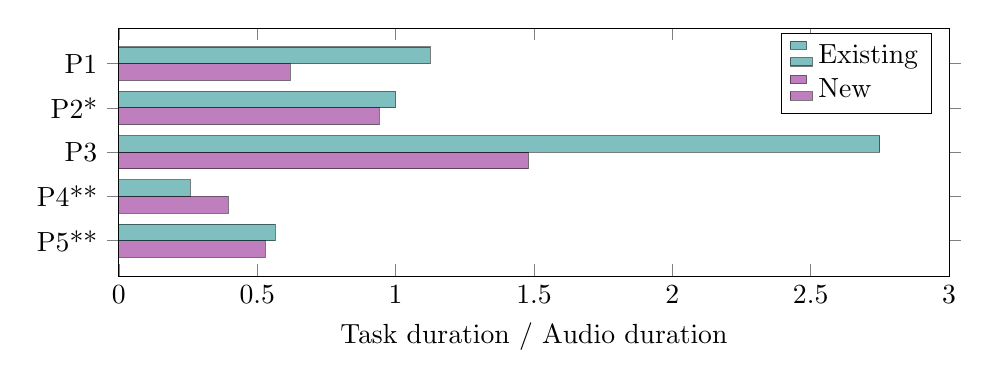
\begin{tikzpicture}
  \begin{axis}[
      width=\columnwidth,
      xbar=0pt,
      bar width=6pt,
      xlabel=Task duration / Audio duration,
      y=16pt,
      xmin=0,
      xmax=3,
      enlarge y limits=0.2,
      symbolic y coords={P1,P2*,P3,P4**,P5**},
      ytick = data,
      y dir=reverse,
      reverse legend,
      legend cell align={left},
      ]
  \addplot[fill=violet, opacity=0.5] coordinates {(0.619,P1) (0.941,P2*) (1.48,P3) (0.395,P4**) (0.529,P5**)};
  \addlegendentry{New}
  \addplot[fill=teal, opacity=0.5] coordinates {(1.125,P1) (1.0,P2*) (2.75,P3) (0.258,P4**)
    (0.565,P5**)};
  \addlegendentry{Existing}
  \end{axis}
  \end{tikzpicture}
  \caption{Time taken to complete the observed task for each workflow, compared to the original audio length. Lower is
    better. *P2 logged their material on paper. **P4 and P5 did not do any logging. Due to the small sample size and
    variation in usage, no conclusions about time performance can be drawn.}
  \label{fig:time} \end{figure}

The time taken to complete the observed tasks was recorded (see Figure~\ref{fig:time}). As various recordings of
different lengths were used for the existing and new workflows, the times are reported relative to the length of the
original unedited audio. In all cases, the producers were able to run the ASR processing as a background
task so this was not included in the calculation. P1, P2 and P3 used the semantic editor after their existing process,
while P4 and P5 did the opposite. However as different recordings were editing on each system, the presentation order
is not expected to affect the results.

The mean average time for semantic editing was 0.79 minutes per minute of audio, versus 1.13 minutes for the existing
method, which is a 44\% improvement. However, a paired \textit{t}-test revealed that there was no statistically
significant difference (\textit{p} = 0.24).  This is due to the small sample size and the large variations in timings
resulting from P4 and P5 not doing any logging, and P2 printing out and annotating their transcript before editing.
Semantic speech editing may have the potential to reduce the time needed for logging and rough-editing material, but
further investigation with a larger sample and consistent workflow is required to measure time performance.

%P2 did go through a logging stage, but did this by printing out the generated transcript and using a highlighter pen
%to select the bits they wanted. This meant that they had to go back and repeat this process using the semantic editor
%interface, which slowed them down. Despite this, the new process was marginally faster.

%P1 and P3 used Dialogger as designed by logging and editing their material using the semantic editing interface. The
%length of their interviews were also much longer, so the benefit of text-based navigation and editing was more
%apparent. In this case, the producers rough edited their material 85\% faster compared to their existing workflow.


\subsubsection{Cognitive load}


%\begin{table}
  %\centering
  %\begin{tabular}{ r | c c c c c | c } & P1 & P2 & P3 & P4 & P5 & Mean \\
    %\hline
    %Mental demand   & -5  & -9  & -2  & 5   & 4 & -1.4 \\ Physical demand & 0   & 4   & 0   & 13  & 0 & 3.4 \\
    %Temporal demand & -1  & 4   & -5  & 4   & 1 & 0.6 \\ Performance     & -2  & 7   & 0   & 2   & 5 & 2.4 \\
    %Effort          & -1  & -7  & 7   & -4  & 2 & -0.6 \\
    %Frustration     & -12 & 1   & -3  & 2   & 5 & -1.4 \\ \hline \end{tabular}
  %\caption{Difference in NASA-TLX results between the old and new workflows.
    %Negative results indicate that the new workflow is better.} \label{tab:tlx} \end{table}

After completing both tasks in the observation, the participants were asked to
rate both the old and new workflows using the raw NASA-TLX metrics
\citep{Hart1988}.
%The results are shown in Figure~\ref{fig:tlx}.
No significant differences were detected for any of the metrics using the paired \textit{t}-test.
With only five participants and marginal differences, it was not possible to
draw any conclusions about cognitive load from these results.  They indicate
that Dialogger requires slightly less effort and mental demand, and is less
frustrating.
However it is considered more physically demanding, temporally
demanding and scores lower in performance.

%To put these results in context, we must look at what the
%participants said in the interviews.

%\begin{figure}
%\centering
  %\begin{tikzpicture}
  %\begin{axis}[
      %width=0.8\columnwidth,
      %height=0.8\columnwidth,
      %bar width=6pt,
      %xbar=0pt,
      %xlabel=Mean TLX value,
      %y=16pt,
      %xmin=0,
      %xmax=100,
      %enlarge y limits=0.15,
      %symbolic y coords={Frustration,Effort,Performance,Temporal demand,Physical demand,Mental demand},
      %ytick=data,
      %legend pos=east,
      %legend style={at={(1,0.5)},anchor=east},
      %reverse legend,
      %]
  %\addplot[fill=violet, opacity=0.5] coordinates {(44.5,Frustration) (53,Effort) (41,Performance) (51.5,Temporal demand) (48,Physical demand) (51,Mental demand)};
  %\addlegendentry{New}
  %\addplot[fill=teal, opacity=0.5] coordinates {(48,Frustration) (54.5,Effort) (35,Performance) (50,Temporal demand) (39.5,Physical demand) (54.5,Mental demand)};
  %\addlegendentry{Old}
  %\end{axis}
  %\end{tikzpicture}
  %\caption{Mean NASA-TLX results for each system. Lower is better.}
  %\label{fig:tlx}
%\end{figure}

\subsubsection{Follow-up usage}
Participants were given access to the system for one month after the study.  The logs from the interface were analysed
to see how the participants used Dialogger during the follow-up stage of the study.

All of the participants continued to use the semantic editor of their own accord as part of their work. The total time
spent by the four remaining participants (P1, P2, P4, P5) using Dialogger in the follow-up period was 23 hours and 58
minutes.  Over 14 hours of those were from P2, with P4 using it for 5 hours, P1 for 3 hours and P5 for 20 minutes.
During this period, 86 recordings were uploaded and 58 audio edits were exported.

%\begin{figure}
%\centering
  %\begin{tikzpicture}
  %\begin{axis}[
      %width=0.8\columnwidth,
      %%height=0.7\columnwidth,
      %bar width=6pt,
      %xbar=2pt,
      %xlabel=User actions,
      %y=11pt,
      %xmin=0,
      %xmax=320,
      %symbolic y coords={Printed edit,Copied edit,Printed transcript,Deleted clip,Copied transcript,Exported audio,Uploaded audio,Re-ordered clip,Created clip},
      %ytick=data,
      %nodes near coords,
      %]
  %\addplot[fill=teal, opacity=0.5] coordinates {(3,Printed edit) (5,Copied edit) (12,Printed
    %transcript) (12,Deleted clip) (22,Copied transcript)
    %(58,Exported audio) (86,Uploaded audio) (178,Re-ordered clip) (270,Created clip)};
  %\end{axis}
  %\end{tikzpicture}
  %\caption{Count of logged user actions during follow-up}
  %\label{fig:actions}
%\end{figure}

Users could navigate the content by either clicking on the waveform or by clicking on a word in the transcript. The
interaction log showed that over 98\% of navigation actions were executed by clicking on a word, which shows a clear
preference for navigating by text compared to waveforms.

%\section{Implications}

%Remove as well as take away

%Annotation is import. Need to include word processing features

%Paper is still used, portable and easy on eyes

\section{Discussion}\label{sec:discussion}
%Two key aims of radio production are to find the most relevant or interesting parts of speech recordings, and
%assemble them into a story.
We found that producers face a number of challenges with audio editing in radio production. There is often a large
quantity of audio to process so it can take a long time. The content of the speech is usually complex and contains
interconnections to things said in other recordings, which can be difficult to keep track of. Making editorial
decisions also requires a high degree of concentration over an extended period, which is demanding, especially in the
noisy and distracting office environment.

We observed that in their existing workflow, participants tackled these challenges by employing a number of techniques
to filter and arrange their audio content. They started by listening back to all of their recordings, which allowed
them to simultaneously assess the editorial content and sound quality of the audio. For long recordings, many
participants `logged' the audio as they listened, by typing rough transcriptions and notes into a word processor, which
they later used to help them edit the audio using a digital audio workstation (DAW). For short recordings, instead of
logging, participants segmented their recordings in the audio editor during playback, and went back to remove unwanted
segments and label the rest.
%Double-speed playback was often used to skim through some of the audio.
All of the participants used a word processor to create a programme script in which they developed the structure and
content of their story. They used annotations to highlight or rate the transcripts, and wrote notes to help them with
selecting and assembling the final content.

We introduced a semantic editing system into professional radio production, which the study participants were able to
successfully use as part of their workflow. On average, the semantic editing workflow was much faster than the existing
workflow, in line with previous findings from \citet{Whittaker2004}, but this result was not statistically significant,
so requires further investigation.  We compared the semantic editing workflow, which included a transcript, to the
existing workflow, which did not. Further research could consider how much benefit is derived from the transcript
itself, compared to the semantic editing interface.  All participants voluntarily continued to use the system after the
trial, which indicates that they found value in using it. However, we identified a number of important features that
were missing or could be used to improve future semantic speech editing systems.

Logging is an important process that primarily involves labelling and organising content, however it is time consuming.
Natural language processing could also be used to assist this process. For example, a text segmentation algorithm
\citep{Choi2000} could divide an interview into different topics, and a keyword extraction algorithm \citep{Matsuo2004}
could provide a summary of what was discussed. However, some participants found the logging process to be valuable
because it gave them the opportunity to listen back through their recordings, and make connections between various bits
of content. This cross-referencing could also be assisted by providing links between words within and between
recordings. For example, selecting a word could display and replay other mentions of that word in other recordings.

Another important reason for listening is to ensure a high `sound quality'. Participants wanted to avoid low quality
audio such as ``umm''s, mumbling, coughing and excessive background noise, but they also wanted to ensure they didn't
miss any high quality audio moments that might not have been identified using the transcript.  Faster playback is
already used in radio production to reduce the time spent listening to material, however more sophisticated time
compression algorithms such as those described by \citet{Arons1997} could be used. Time compression has not been
included in previous semantic editing systems, but should be considered in the future, especially as \citet{Vemuri2004}
found that the maximum time compression factor is significantly higher when an automated transcript is present.

Removal of ``umm''s and breaths, known in radio production as `de-umming', is either done by the producer themselves or
with the help of a sound engineer, depending on the producer's experience and time pressure. To maintain sound quality,
the removal of umms/breaths must be audibly transparent and participants reported that this can difficult to achieve.
Previous semantic editing systems have included functionality to remove umms \citep{Berthouzoz2012} and breaths
\citep{Rubin2013}, however these were made possible because the manually generated transcripts 
explicitly transcribed those items. ASR systems are normally trained to ignore umms/breaths rather than
transcribe them, which prevented us from including this functionality. A transcription system that includes these would
allow us to add this functionality, however further research is needed into the extent to which de-umming can be
automated in this way.

All of the participants used a script document to structure and assemble their programme, and as a
medium to inform and gather feedback from the presenter about the content and layout of the programme. Although the
clipboard of our semantic editing system acted much like a programme script, the participants did not use it in that
way because it was missing some key functionality for annotation and collaboration.

Annotation features were an important requirement that we did not pick up on during the design specification, and which
have not been included in previous semantic speech editing systems. Two participants in our study deviated from the
expected workflow in order to annotate the transcript, and the other participants noted the absence of such
functionality. Participants wanted to be able to annotate the transcripts as they would with a word processor, in order
to highlight or rate particularly good parts of their recordings, add personal comments, and to segment and label the
content.

A simple change to achieving this would be to allow the transcripts to be formatted, and for textual comments to be
inserted and edited. Furthermore, the drag-and-drop editing could be replaced with cut/copy/paste similar to
\citet{Whittaker2004} and \citet{Rubin2013}. An alternative approach could be to add semantic speech editing
functionality to a word processor, rather than adding word processing functionality to a semantic speech editor.

Scripts are used as a tool for collaborating with colleagues such as the
presenter because the programme's content and structure can be quickly reviewed and
commented on by others without them having to spend time downloading and listening to the audio. Our semantic editing
system was designed for individual access to transcripts and edits, however this meant that they could not be shared
with the presenter. A better approach would be to allow multiple users to navigate and edit the same material. This
could be achieved using operational transformation \citep{Sun2004} which can support concurrent users editing the same
content. Participants were also interested in tighter integration with the DAW. The same technology could be used
to create bi-directional integration with DAWs, so that any edits made in the DAW are automatically updated in the
semantic editor and vice-versa.
%Collaborative annotation features such as those explored by \citet{Yoon2014} could also
%be integrated.

Participants reported that the open-plan office environment in which they worked was often noisy and distracting, and
that they had difficultly working on screens for extended periods. As a result, many reported that they work from home
to get away from the office or print transcripts so they can get away from the screen. A more portable semantic speech
editing system would allow producers the flexibility to work where they wanted.

Digital pen interfaces such as the Anoto system could be used to create a paper-based semantic editor that can be used
anywhere and does not involve screens. Additionally, it naturally supports freehand annotation and may be a better
medium for face-to-face collaboration.  \citet{Klemmer2003} has previously explored how speech can be navigated using
paper transcripts and \citet{Weibel2008} describes how an Anoto system can be used to edit digital documents, however
these approaches have yet to be combined.

Participants reported that the automatically-generated transcripts were sufficiently accurate for editing, supporting
similar previous findings from \citet{Whittaker2004} and \citet{Sivaraman2016}. This is helped by the fact that radio
producers record the audio themselves, and can use their memory to cope with inaccuracies. Most participants were only
interested in correcting errors that were distractingly wrong, which were often names or locations related to the
story. However, as these are known ahead of time, they could be provided to the ASR system as a way to tweak
or expand the language model.

Currently transcripts of each programme are not published due to the high cost and
overhead, however several participants were interested in fully correcting their transcripts so they could do this.
The availability of ASR transcription could have the potential to extend the scope of radio production to include
publication of transcripts. This could help to improve discoverability of programme content, especially if word timings
were included.

% Intro
% What we tested on who, and why

% Sound quality
%   Producers said they need to listen. What for?
%   Time compression could be used to reduce listening time.
%   Automatic detection/removal of umms and breaths could be added to STT systems.
%   Could incorporate sound effect detection.
%\subsection{Sound quality}

% Skepticism about success of automatic removal?  Pauses?

% Structure
%   Labels are often used to organise recordings during logging Natural language processing could be applied to segment
%   and label content

% Collaboration Producers use scripts to structure their programme Producer works closely with the presenter. Needs
% sign-off from editor.
%   Interface could be expanded to support collaboration with audio integration. e.g. Google Docs style interface
%   Document centric collaboration

% Portability
%   Office is noisy, screens are hard on the eyes, so people work from home or outside office
%   Paper-based interface could be used to edit transcript away from desk and screen

% Correction
%   Generally transcripts are good enough to edit with, but participants wanted to correct distracting errors
%   Most participants suggested providing the speech-to-text system with prior information (e.g. names) to reduce errs

% Demand
%   Producers continued using the interface after the investigator left
%   The system is being developed into a supported production tool, which demonstrates its value

% Time
%\citet{Whittaker2004} previously found that semantic editing is faster and as accurate as waveform-based editing for
%voicemail. Our results indicate that semantic editing is potentially faster for radio production, however our sample
%size was not large enough to draw any conclusions.

% Others didn't test properly, we did
%Previous work on transcript-based media interfaces introduced a range of novel
%features for semantically navigating and editing audio and video content.  \citet{Whittaker2004} showed that for
%voicemail content, semantic editing using automatic transcripts was faster and as accurate as waveform-based editing.
%\citet{Casares2002}, \citet{Berthouzoz2012} and \citet{Rubin2013} all created similar systems for audio and video
%production, but they used perfect transcripts and did not perform any formal
%studies on the semantic editing features. In this paper, we presented a semantic speech editor that was designed
%specifically for radio producers based on the results of a pilot study. We studied the existing workflow and evaluated
%the impact of the semantic editor through a qualitative study of five professional radio producers.

% Logging and rough editing is boring
%We found that for production of factual radio programmes, a significant amount of time is spent `logging' speech
%recordings by transcribing them by hand and making notes. This process helps the producer to select the best bits of
%their
%material and to structure the narrative of their programme. After logging,
%producers create a rough edit by using an audio editor to pick out each piece of audio they want, guided by the
%timestamps in their notes. However, these processes take a long time, require concentration, and are considered to be
%boring and tedious.

% Our system was much faster, so frees up their time for other things
%Our semantic editing system `Dialogger' introduced automatically-generated
%transcripts, which meant that the participants could log their recordings much
%faster.  Additionally, the interface allowed them to edit the audio directly
%from the transcript, bypassing the rough edit stage, and saving additional
%time. Freeing-up this time would allow the producers to concentrate on more
%valuable activities such as background research, finding contributors, or
%recording additional material. In turn, this could have the potential to
%improve the editorial quality of the programme.

% Most of the benefit is from the transcript itself, but how much?
%In our experiment, the automatic transcription and the editing interface were
%tested as a whole. However, many participants suggested that most of the
%benefit derived from the system came from the automatic transcription. A future study could test these aspects
%separately to investigate the proportional time saved by the transcription compared to the interface itself.

% The transcripts aren't perfect, but they're good enough to edit when you can
% listen
%As the transcripts were automatically-generated, approximately 16\% of the words were inaccurate. Despite this, most
%participants found them to be sufficiently accurate for their purposes, which supports the findings from voicemail
%editing \citep{Whittaker2004} and voice-based discussions \citep{Sivaraman2016}. 

% Even if the transcript is perfect, producers still need to listen
%In theory, if the transcripts were perfect, it would be possible to rough cut recordings without having listened to
%them. However, a verbatim transcript cannot tell you whether something was said seriously or in jest, or about
%emphasis, cadence, intonation or background noise. Therefore, an interface that
%allows users to edit speech based purely on the transcript carries the risk of creating poor quality results. It is
%important for such systems to make it easy for users to listen to parts of the transcript so they can determine the
%quality of the audio they are editing.

% Transcripts need correcting to be readable on their own
%Although the automatic transcripts were considered good enough to edit with, the producers often had to listen to parts
%of the recording to make sense of
%them. If the transcripts are to be used independently of the audio, the
%producer must have an easy way to fix the mistakes. Rather than make the user type out each replacement word, this
%process could be aided by allowing them to select alternative words that were rejected by the speech-to-text system.

% Many producers like working on paper, but need to listen to make sense
%Despite the importance of listening, many producers like to work on paper.
%Participants said that they enjoyed being able to work away from the desk, that it was easier on their eyes, and that
%it was easier to collaborate with others using printed documents. However, when transcripts are printed, the timing
%information which links the words to the audio is lost. It would be feasible 
%to develop a system for moving between paper and the screen which could
%retain this information, but no such existing system could be found.

% Annotation helps the producer to mark their favourite bits
%The role of the transcripts is ultimately to help the producer pick which bits
%of audio to use in their programme. To achieve this, they use annotations to
%mark and rate segments of the transcript. This functionality has not been
%considered in any previous semantic editing systems, but we found it to be an
%important feature which participants went out of their way to replicate.

%In creating and testing Dialogger, we found that there was demand for semantic
%editing in radio production. This was backed up by the continued use of the
%system during the follow-up period, which was unprompted.
%During the study, many of the radio producers reported that a similar
%transcript-based workflow exists in television production. Due to the high
%costs of video editing, transcripts are often used to make editorial decisions
%before editing begins. It would be interesting to see if a semantic video
%editor would bring similar benefits to a television production workflow.

% What did you learn from making the system?

% What does this tell us about these kinds of systems?
%- Mature enough to be used in professional practice


% How does this impact the workflow?

% How does this impact the job role?


% Television


% How does this impact the nature of programme making


%CONTIBUTIONS COMPARED TO OTHER WORK

%Logging helps producers to recall what was said in interviews and to structure and cross-reference

%Logging takes a long time, requires concentration and is boring.

%Producers annotate the logs with timestamps, notes, highlighting and star ratings.

%Word is used and preferred for making annotations

%Navigation using a transcript is considered faster

%There is a desire to listen to the audio faster than real time

%The transcript is accurate enough to do a rough edit

%A more accurate transcript would be beneficial

%The transcript interface is not needed for short recordings or fine editing

%Drag and drop clipping didn't work very well as it's hard to select long bits

%There is a desire for cut and delete functionality

%Working on paper is desirable

%Television could also benefit from this approach

%Need to listen to the audio

%Task completed up to twice as fast with the new system when including logging

%Participants continued to use the prototype after the study

%\subsection{Recommendations}

%\paragraph{Word processing}
%The participants in our study made heavy use of word processing software to filter and arrange their speech recordings
%by using the editing and annotation features. For radio production, semantic speech editors should replicate, or
%integrate with, word processing functionality.

%\paragraph{Collabotation}
%Radio production involves working with others, so semantic speech editors should include features for collaborative
%working. Making use of operational transformation techniques would allow concurrent editing with multiple users, and
%integration with multiple interfaces.

%\paragraph{Portability}


%\paragraph{Sound quality}


\subsection{Outcome}
Based on the results of this work, we developed the prototype further to take into account the feedback from the
producers in our study.  We handed the prototype over to a development team at the BBC who have now turned it into an
officially supported production tool.  This has allowed producers from around the BBC to use the tool as part of their
normal workflow.
As of October 2016, the system had 45 active users and has processed 265 audio recordings.
%We will continue to collect usage and interaction metrics for later analysis.

%In further research work we have added the ability to print augmented paper transcripts, whose annotations result in
%automatic edits to the source audio. This was done in a collaboration between the BBC and Anoto, and is currently being
%evaluated against screen-based editing in a further study.

%\subsection{Summary of main findings}\label{sec:findings}
%used a pilot study to identify an opportunity to use automatic transcripts of
%dialogue with synchronised audio to connect two previously separate activities
%in radio editing. This had mixed results as shown by the weak stats but more
%positive comments. It exposed some important missing functions like annotation
%and the importance of paper. The exercise also seems to have resulted n the
%first published study of documentary radio production.

% start with a summary and then extend each element at greater length

%\paragraph{There is demand for semantic editing in radio production}
%In the follow-up stage of the study, all of the participants continued to use
%the semantic editing interface of their own accord as part of their production workflow. This result demonstrates that
%they find the interface beneficial to their practice. The interface has also been developed into a supported
%production tool which also demonstrates that there is a business case in making
%this available to production staff.

%\paragraph{Semantic editing is faster for long recordings}
%For editing short audio content ($\sim$10 mins), or when editing without
%logging, we found that there was no speed benefit in using semantic editing. However, logging and rough editing longer
%recordings using the semantic editing workflow was completed up to twice as fast as the existing workflow. Participants
%also commented that the semantic editing system felt much faster to use and allowed them to quickly search and
%cross-reference the
%material.

%\paragraph{Automatic transcriptions are sufficiently accurate} The participants in the study used
%automatically-generated transcripts to navigate and edit the audio. Even though the transcripts had a word error rate
%of approximately 16\%, they were found to be sufficiently accurate for the purposes of radio production.  This supports
%similar findings about semantic editing of voicemail content from \citet{Whittaker2004} and of voice-based
%discussions from \citet{Sivaraman2016}. However, the more accurate the transcripts are, the better.

%\paragraph{Annotation features are important} Participants annotated their logs with timestamps and notes, and used
%star
%ratings and highlighting to indicate important parts of their recordings. As
%this functionality was not included in the semantic editing interface, some participants imported the transcripts into
%MS Word to allow them to make these annotations.  This demonstrates that annotation is an important feature to include
%in such systems.
%This broke the connection between the audio and the text.
%These annotation features could be added to the semantic editing system which
%would allow the audio and transcript to remain linked.

%\subsection{Drag-and-drop doesn't work} The interface was designed so that users could select desired pieces of
%content using a drag-and-drop technique. This design worked well for short clips, but could not handle long clips. In
%addition to selecting content they did want, participants were also interested in removing content that they didn't
%want.  Enabling word processor style editing like cut, copy and paste would give the users more freedom.
%%TODO SO...

%\paragraph{Producers want to work on paper} The participants often used paper to read and annotate their scripts and
%logs because it was easier on their eyes, helped them to collaborate and allowed them to be productive away from the
%desk, such as in caf\'{e}s and on trains.  During the study, one participant printed the transcript from the semantic
%editing interface and worked on paper, even though this meant having to go back to find and create the desired clips.

%went out of their way to edit on paper by printing and highlighting the transcript.  Being able to move between the
%screen and paper would bring the benefits of paper working and allow producers to use their time more efficiently.

%\paragraph{Listening is important} Finally, participants pointed out that ``radio is made with your ears''.  Editing
%decisions are based not only on what is said, but how it is said. This emphasises the importance of a multi-modal
%interface, which combines the efficiency of text-based working with being able to quickly listen back to the audio.
%Enhancing this with faster than real time listening would allow users to review material at much faster speeds than
%they do already \citep{Vemuri2004}.


\section{Conclusion}\label{sec:conclusion}
We conducted a contextual study of semantic speech editing in professional radio production. The participants were able
to use our system to produce real programmes and they continued to use it after the study.  However, the results
highlighted a number of opportunities to better address the needs of radio producers.
Annotation features such as highlighting, ratings and comments are needed to aid producers in organising and
structuring their content.
Radio production is a collaborative process, so semantic editing tools should support multiple users. Use of
operational transformation would allow concurrent editing and integration between multiple interfaces.
Some participants struggled with office and screen-based working so portable interfaces, such as those offered by
digital pen technology, would give producers the flexibility to work where they are most productive. 
Unwanted noises such as `umms' and breaths must be removed transparently, which is done by the producer or sound
engineer. By training ASR systems to transcribe these noises, this could be done in the semantic editor.
However, further research is required into the sound quality achieved by this approach.
Finally, ``radio is made with your ears'' so there are limits to how much editing can be done using a text-based
interface. Editing tools should provide easy access to playback and use time compression features, which allow users to
listen much faster, particularly in combination with the transcript.

%Semantic editing of speech has direct applications in professional audio production, but previous studies of such
%systems were informal and used amateur participants. We developed a semantic speech editing system based on the
%results of a pilot study of radio production, and conducted a formal user study of the system with five producers at
%the BBC.  We used speech-to-text to generate transcripts, which were accurate enough to allow the producers to
%rough-edit their recordings up to twice as fast as their current method.  During the study, we discovered that
%annotating the transcript is an important part of the editing process, and that producers enjoy working on paper.
%Although it is possible to use these systems to edit audio using only a transcript, we found that it cannot replace
%listening to the audio. After the study, the producers continued to use the system, which has since been developed
%into a supported BBC production tool after receiving investment.

